\documentclass{beamer}

\usepackage{hyperref}
\usepackage{graphicx}
\usepackage{tikz}
\usepackage{xcolor}
\usetikzlibrary{calc}

\newcommand{\NH}{\text{NH}}
\newcommand{\RG}{\text{RG}}

\title{Measuring the Price of Anarchy in Critical Care Unit Interactions}
\author{Vincent Knight and Izabella Komenda}
\date{2014-07-25}

\setbeamertemplate{navigation symbols}{}

\begin{document}

\frame{
    \Huge
    \[
        \begin{pmatrix}
        (2,2)&(5,0)\\
        (0,5)&(4,4)
        \end{pmatrix}
    \]
}

\frame{

\begin{columns}
\column{.5\textwidth}
\begin{itemize}
\item $k=1$
\item $\mathcal{P}_1=\{1,2\}$
\item $c_1=1$ and $c_2=x$
\item $r=1$
\end{itemize}
\column{.5\textwidth}

\includegraphics[width=5cm]{./Images/PigousExample.pdf}
\end{columns}\vspace{.5cm}
The Nash flow minimises:
\begin{align}\Phi(y,1-y)&=\sum_{e=1}^2\int_{0}^{f_e}c_e(x)dx=\int_{0}^{y}1dx+\int_{0}^{1-y}xdx&\nonumber\\
&=y+{(1-y)^2\over2}={1\over2}+{y^2\over 2}\nonumber\\
&\Rightarrow\tilde f=(0,1)\nonumber
\end{align}
}

\frame{
\begin{center}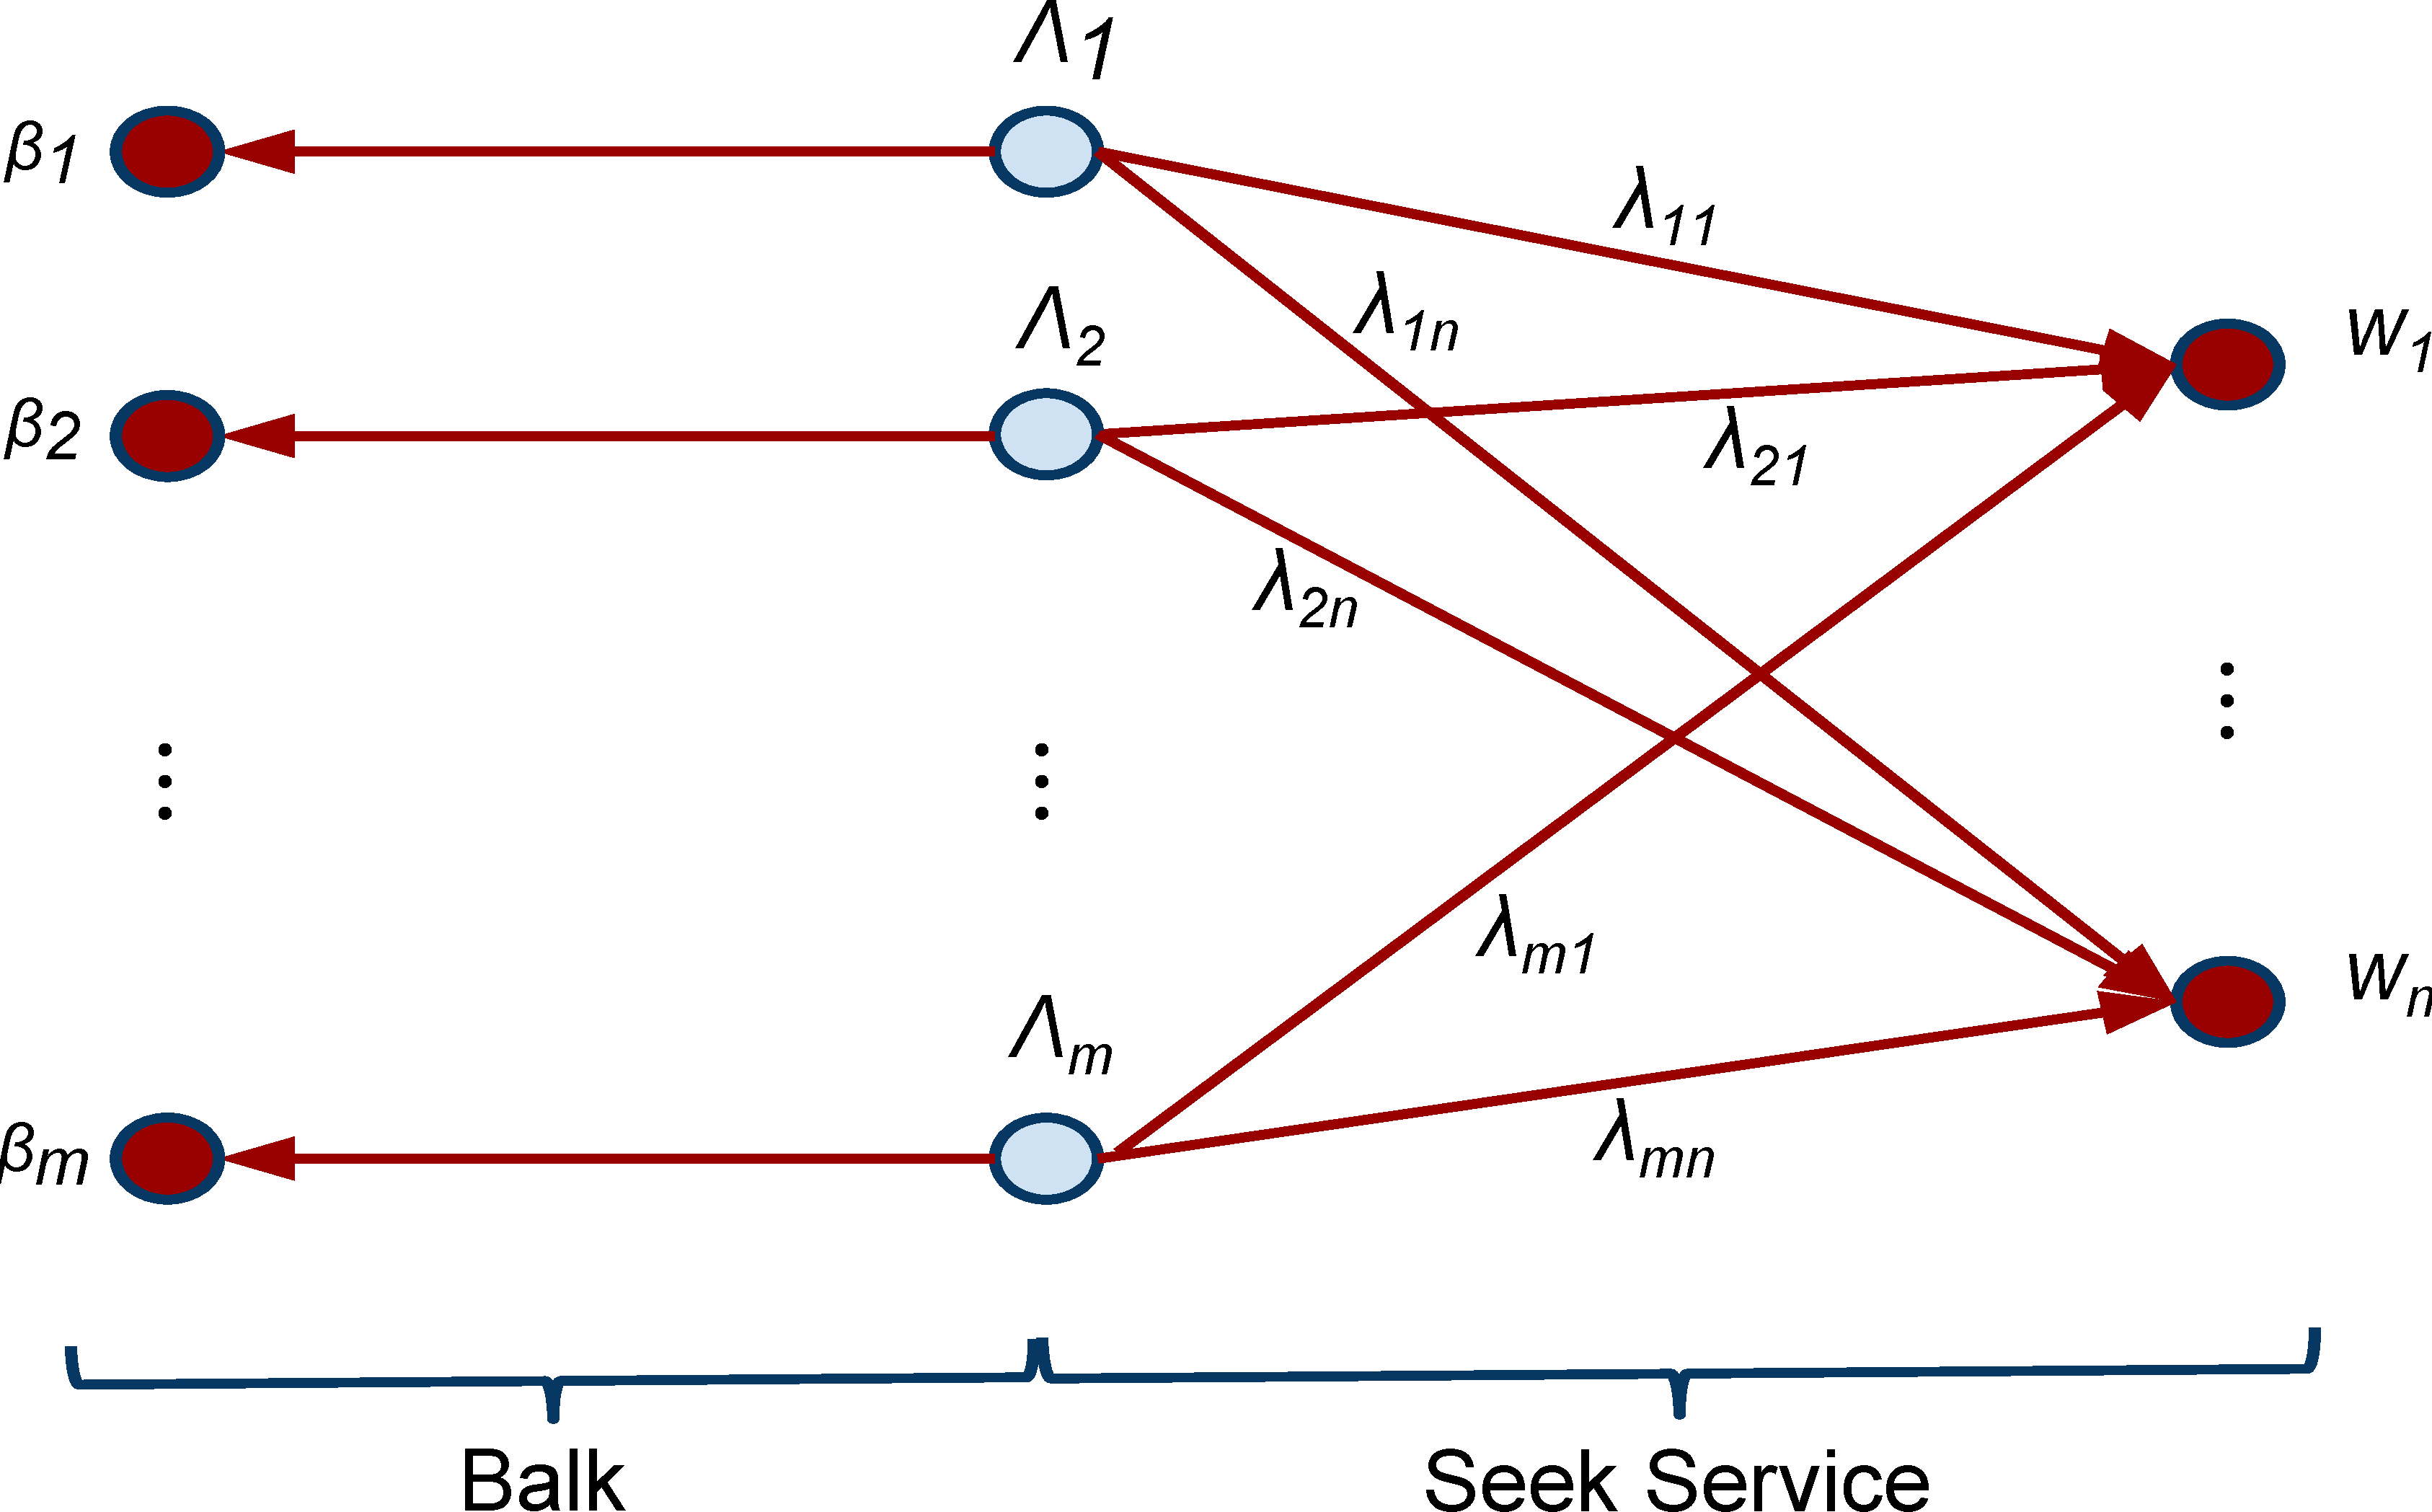
\includegraphics[width=10cm]{./Images/Hospital_Choices.pdf}\end{center}}

\frame{
\begin{columns}
\column{.25\textwidth}
\begin{itemize}
\item $k=m$
\item $\left|\mathcal{P}_i\right|=n+1$
\item $r_i=\Lambda_i$
\end{itemize}
\column{.75\textwidth}
\only<1>{\begin{center}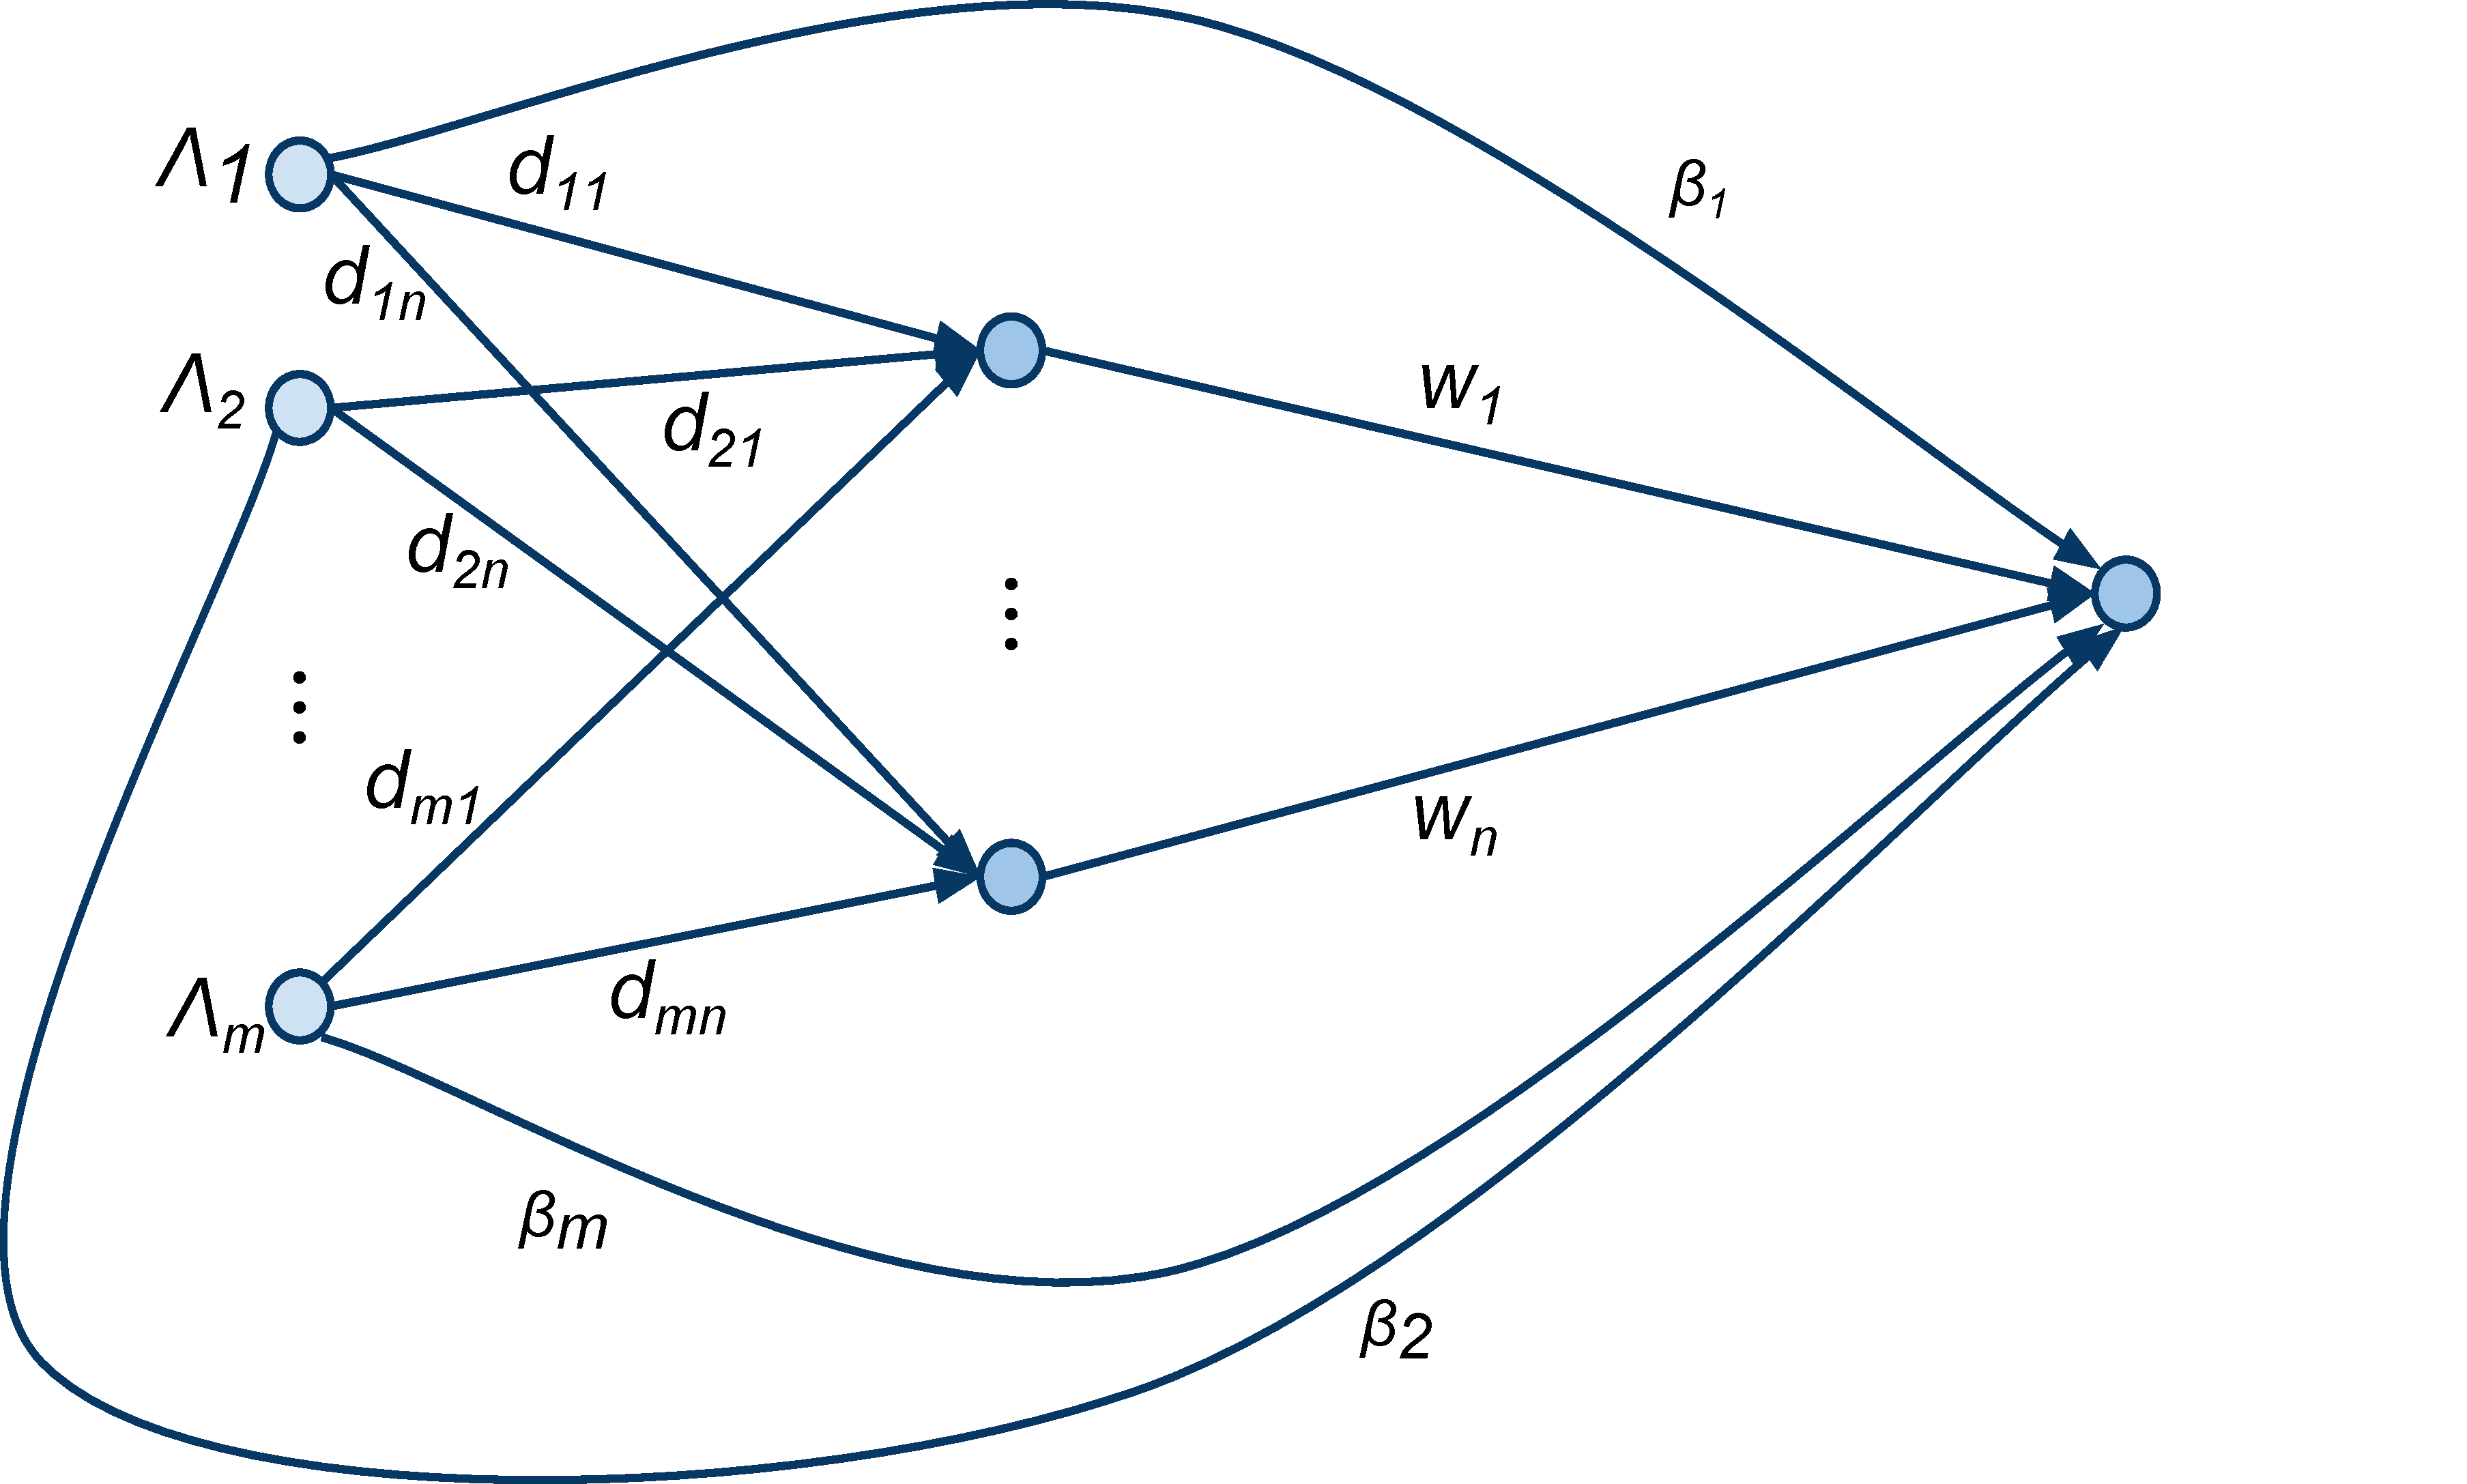
\includegraphics[width=8.5cm]{./Images/Hospital_Routing_Game.pdf}\end{center}}
\only<2>{\begin{center}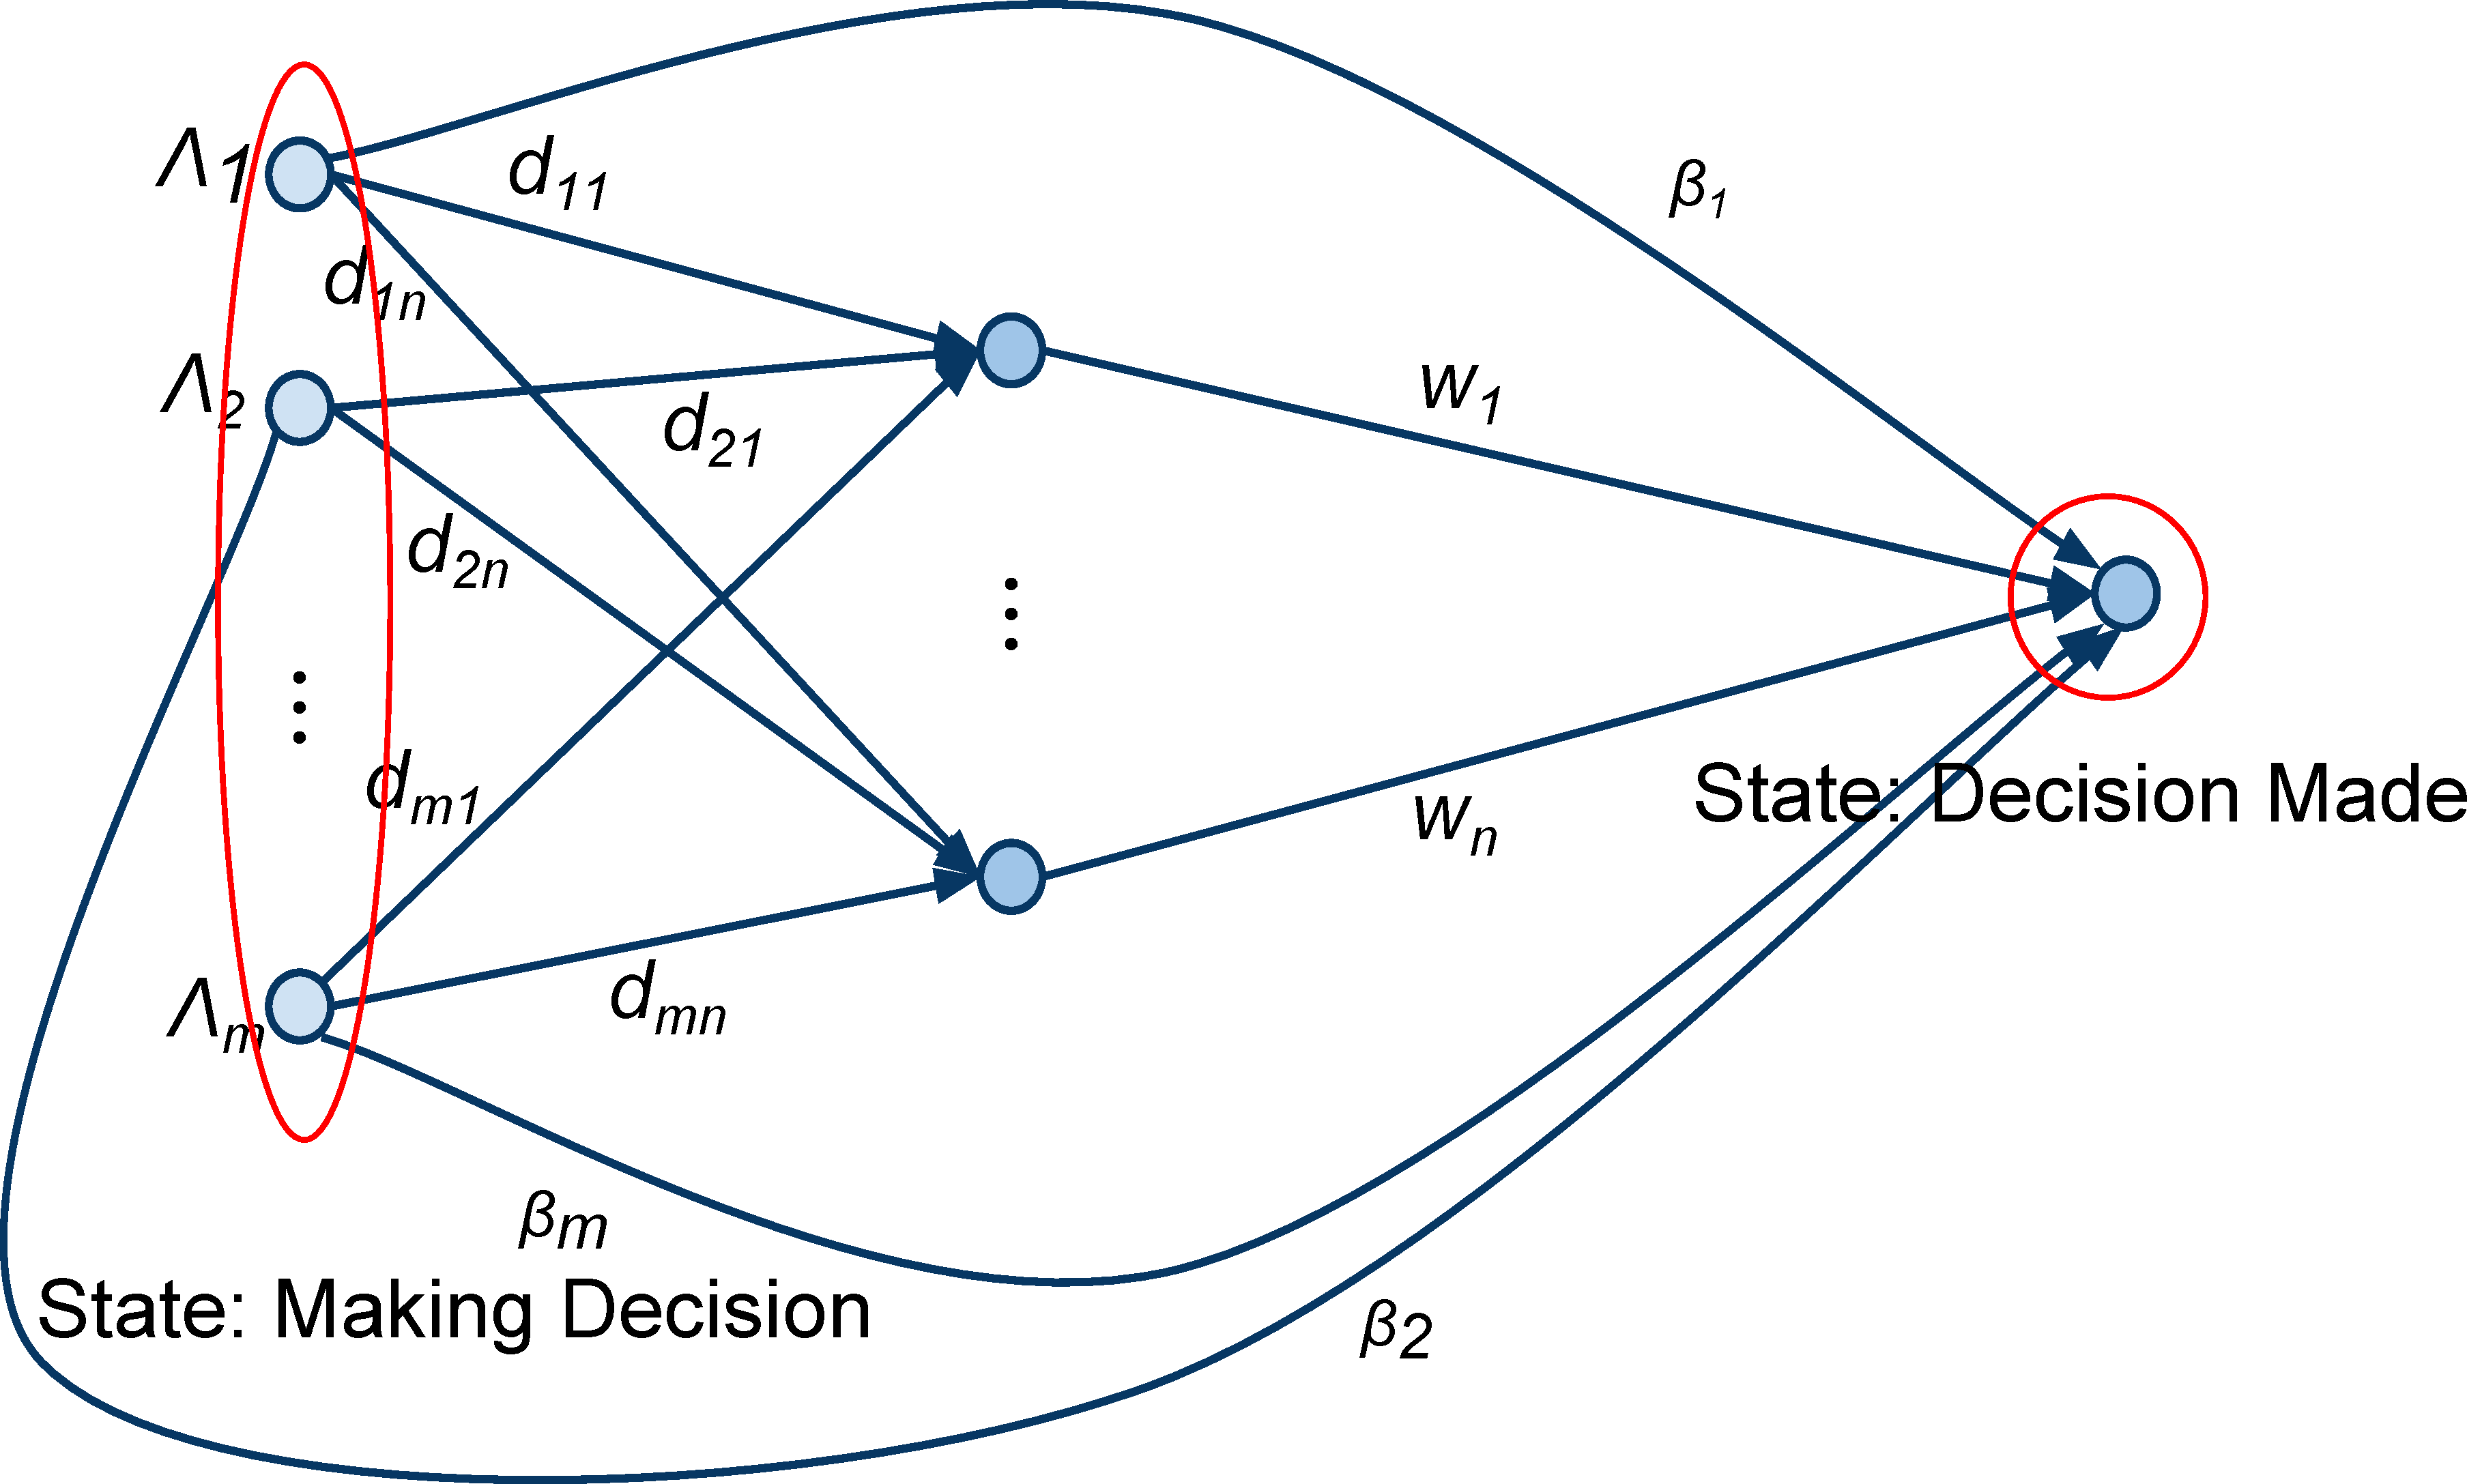
\includegraphics[width=8.5cm]{./Images/Hospital_Routing_Game_1.pdf}\end{center}}
\end{columns}}

\frame{
\textbf{Theorem}
Assuming $\sum_{i=1}^{m}\Lambda_i<\sum_{j=1}^nc_j\mu_j$ we have:
$$\lim_{\beta_i\to\infty}PoA(\beta)<\infty\text{ for all }i\in[m]$$
\begin{center}\it{The price of anarchy increases with worth of service, up to a point.}\end{center}
\textbf{Proof.}
\begin{itemize}
\item$ \lim_{\beta_i\to\infty}\lambda^*=k^*$ and $ \lim_{\beta_i\to\infty}\tilde\lambda=\tilde k$
\item As $\beta_i\to\infty$: $$\sum_{i=1}^m\Lambda_i=\sum_{i=1}^m\sum_{j=1}^n\lambda^*_{ij}=\sum_{i=1}^m\sum_{j=1}^n\tilde \lambda_{ij}$$
\item $PoA(\beta)<\infty$
\end{itemize}
}

\frame{
    \begin{center}
        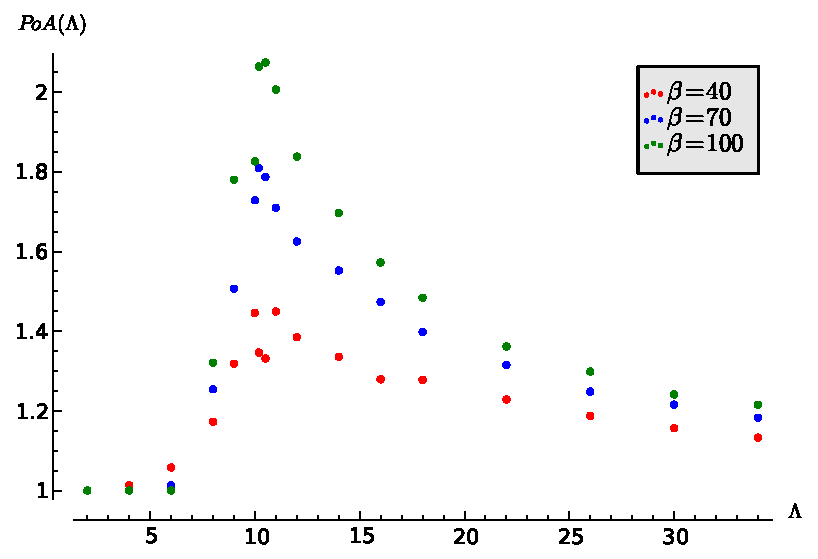
\includegraphics[width=.8\textwidth]{./Images/PoA_Healthcare.pdf}
    \end{center}
}
\frame{
        \textbf{Price of Anarchy in Public Services} \textit{EJORS}, 2013.
}


\frame{
    \begin{center}
        {\Huge What about the controllers?}\\
        \vspace{1cm}
    \end{center}
        \pause
        S. Deo and I. Gurvich. \textbf{Centralized vs. Decentralized Ambulance Diversion: A Network Perspective.} \textit{Management Science}, May 2011.
}

\frame{
    \begin{center}
        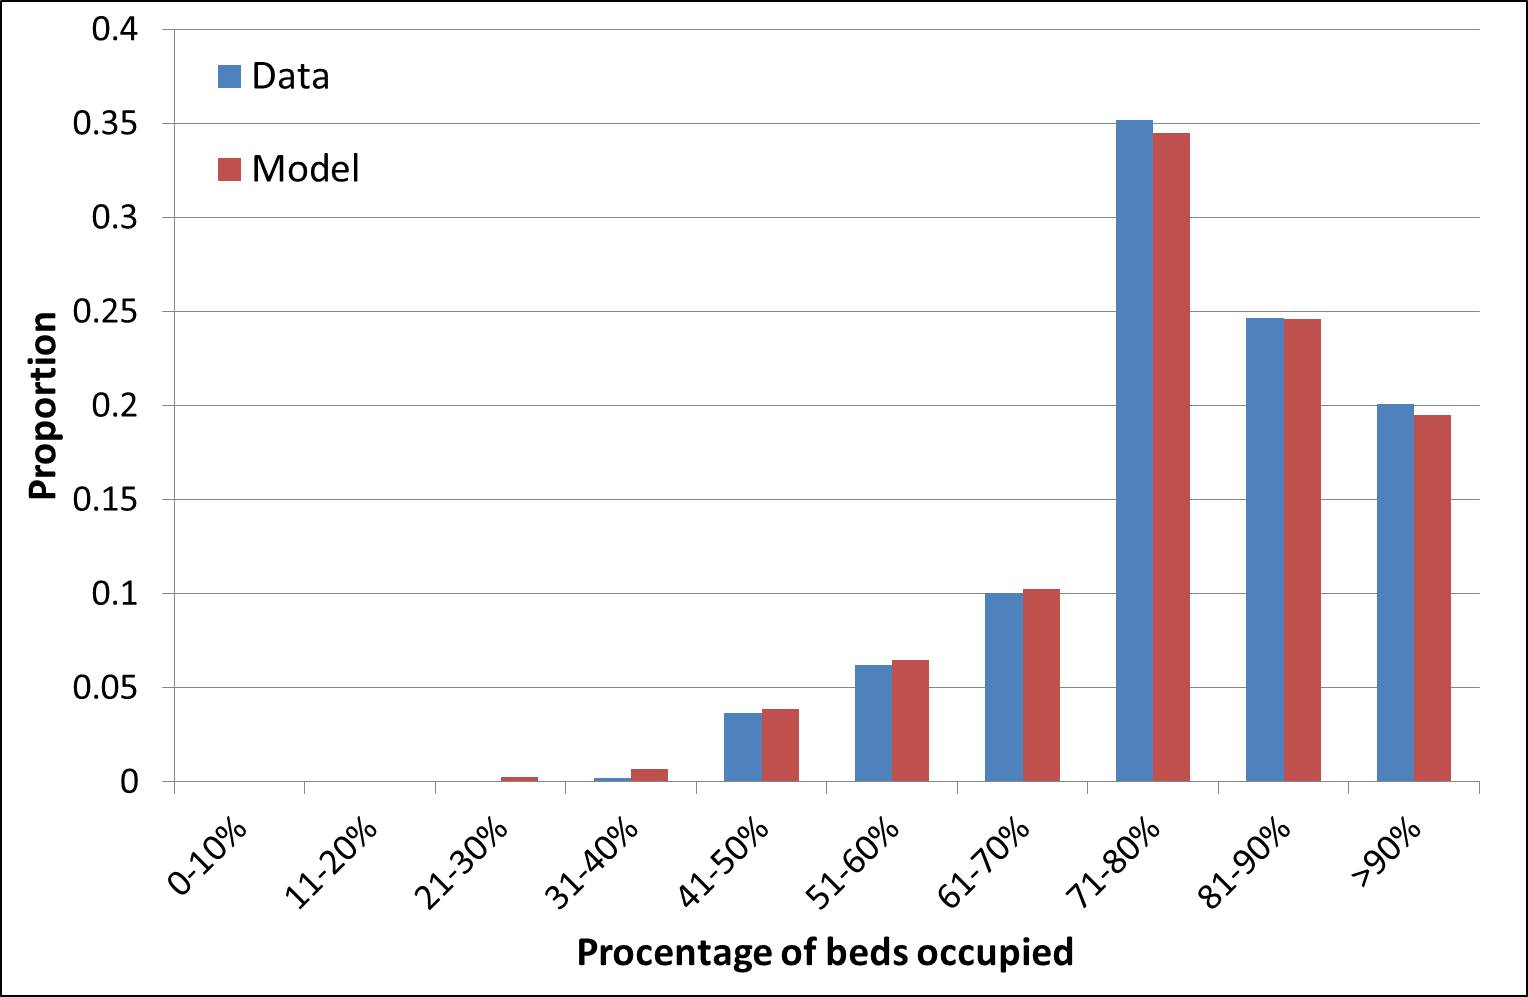
\includegraphics[width=.8\textwidth]{./Images/RG_state_dependent_model.jpg}
    \end{center}
    \pause
    \textbf{Mathematical modelling of patient flows to predict critical care capacity required following the merger of two District General Hospitals into one.}, \textit{Submitted to Anaesthesia}
}

\frame{
\begin{center}
    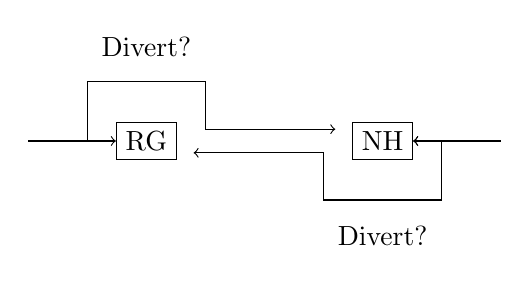
\begin{tikzpicture}[scale=1.5]
        \node (A) at (0,0) [draw] {RG};
        \node (B) at (2,0) [draw] {NH};
        \draw [->] (-1,0) -- (A);
        \draw [->] (3,0) -- (B);
        \draw [->] (-1,0) -- ($(A)+(-.5,0)$) -- ($(A)+(-.5,.5)$) -- ($(A)+(.5,.5)$) -- ($(A)+(.5,.1)$) -- ($(B)+(-.4,.1)$);
        \draw [->] (3,0) -- ($(B)+(.5,0)$) -- ($(B)+(.5,-.5)$) -- ($(B)+(-.5,-.5)$) -- ($(B)+(-.5,-.1)$) -- ($(A)+(.4,-.1)$);
        \draw [->] (3,0) -- (B);
        \node at ($(A) + (0,.8)$) {Divert?};
        \node at ($(B) + (0,-.8)$) {Divert?};
    \end{tikzpicture}
\end{center}
}

\frame{
\begin{center}
    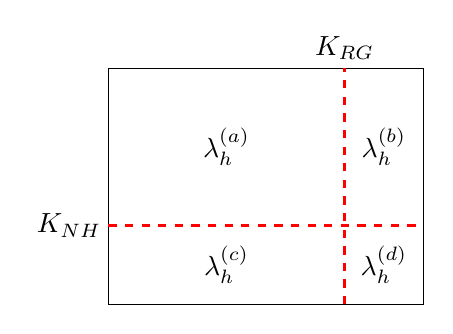
\begin{tikzpicture}
        \draw  (0,0) rectangle (4,3);
        \draw [dashed, red, thick] (0,1) -- (4,1);
        \draw [dashed, red, thick] (3,0) -- (3,3);
        \node at (-.5,1) {$K_{\NH}$};
        \node at (3,3.25) {$K_{\RG}$};
        \node at (1.5,2) {$\lambda_{h}^{(a)}$};
        \node at (3.5,2) {$\lambda_{h}^{(b)}$};
        \node at (1.5,.5) {$\lambda_{h}^{(c)}$};
        \node at (3.5,.5) {$\lambda_{h}^{(d)}$};
    \end{tikzpicture}
\end{center}
}

\frame{
\begin{center}
    \only<1>{
        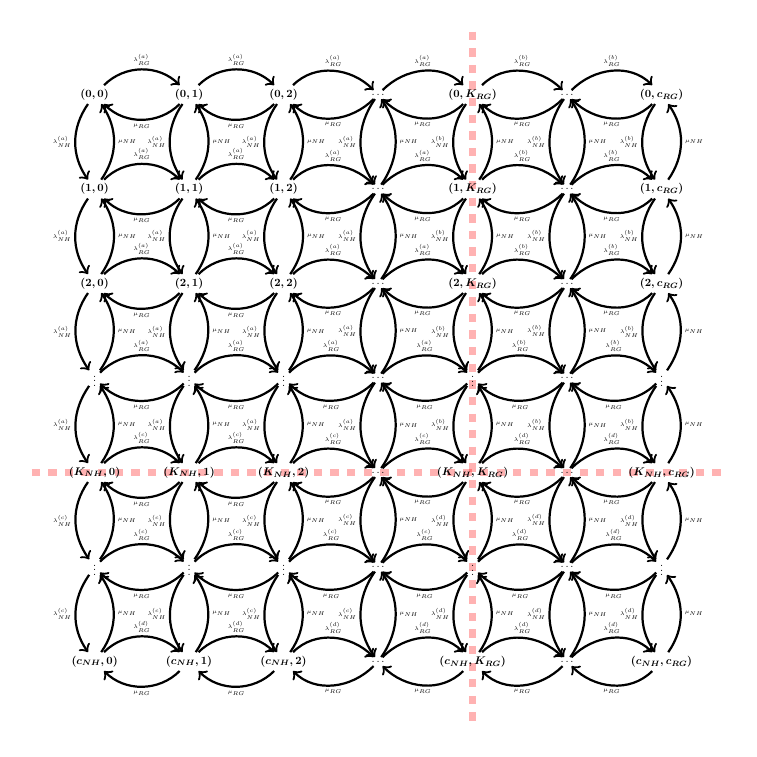
\begin{tikzpicture}[scale=.4, every node/.style={scale=0.4}]
    % -----------------------------------------------
    % Boundaries ------------------------------------
    % -----------------------------------------------
    \draw [dashed, line width=1mm, red, opacity=.3] (12,2) -- (12,-20);
    \draw [dashed, line width=1mm, red, opacity=.3] (-2,-12) -- (20,-12);
    %\tikzstyle{state}=[ellipse, draw, fill=blue!10, minimum width=2cm];
    %\tikzstyle{state}=[rectangle, draw, fill=blue!10, minimum width=2cm];
    \tikzstyle{state}=[minimum width=2cm, font=\boldmath];
    %\draw  (0,0) rectangle (4,3);
    %\draw [dashed, red, thick] (0,1) -- (4,1);
    %\draw [dashed, red, thick] (3,0) -- (3,3);
    % -----------------------------------------------
    % First row--------------------------------------
    % -----------------------------------------------
    \node (aa) [state] at (0,0) {$(0,0)$};
    \node (ab) [state] at ($(aa) + (3,0)$) {$(0,1)$};
    \node (ac) [state] at ($(ab) + (3,0)$) {$(0,2)$};
    \node (ellipsisa1) at ($(ac) + (3,0)$) {$\dots$};
    \node(ak) [state] at ($(ellipsisa1) + (3,0)$) {$(0,K_{\RG})$};
    \node (ellipsisa2) at ($(ak) + (3,0)$) {$\dots$};
    \node(az) [state] at ($(ellipsisa2) + (3,0)$) {$(0,c_{\RG})$};
    % Transitions -----------------------------------
    % On Row:
    \draw (aa) edge[out=45,in=135,->,thick] node [above] {\tiny$\lambda_{\RG}^{(a)}$} (ab);
    \draw (aa) edge[out=-45,in=-135,<-,thick] node [below] {\tiny$\mu_{\RG}$} (ab);

    \draw (ab) edge[out=45,in=135,->,thick] node [above] {\tiny$\lambda_{\RG}^{(a)}$} (ac);
    \draw (ab) edge[out=-45,in=-135,<-,thick] node [below] {\tiny$\mu_{\RG}$} (ac);

    \draw (ac) edge[out=45,in=135,->,thick] node [above] {\tiny$\lambda_{\RG}^{(a)}$} (ellipsisa1);
    \draw (ac) edge[out=-45,in=-135,<-,thick] node [below] {\tiny$\mu_{\RG}$} (ellipsisa1);

    \draw (ellipsisa1) edge[out=45,in=135,->,thick] node [above] {\tiny$\lambda_{\RG}^{(a)}$} (ak);
    \draw (ellipsisa1) edge[out=-45,in=-135,<-,thick] node [below] {\tiny$\mu_{\RG}$} (ak);

    \draw (ak) edge[out=45,in=135,->,thick] node [above] {\tiny$\lambda_{\RG}^{(b)}$} (ellipsisa2);
    \draw (ak) edge[out=-45,in=-135,<-,thick] node [below] {\tiny$\mu_{\RG}$} (ellipsisa2);

    \draw (ellipsisa2) edge[out=45,in=135,->,thick] node [above] {\tiny$\lambda_{\RG}^{(b)}$} (az);
    \draw (ellipsisa2) edge[out=-45,in=-135,<-,thick] node [below] {\tiny$\mu_{\RG}$} (az);
    % -----------------------------------------------
    % Second row--------------------------------------
    % -----------------------------------------------
    \node (ba) [state] at (0,-3) {$(1,0)$};
    \node (bb) [state] at ($(ba) + (3,0)$) {$(1,1)$};
    \node (bc) [state] at ($(bb) + (3,0)$) {$(1,2)$};
    \node (ellipsisb1) at ($(bc) + (3,0)$) {$\dots$};
    \node(bk) [state] at ($(ellipsisb1) + (3,0)$) {$(1,K_{\RG})$};
    \node (ellipsisb2) at ($(bk) + (3,0)$) {$\dots$};
    \node(bz) [state] at ($(ellipsisb2) + (3,0)$) {$(1,c_{\RG})$};
    % Transitions -----------------------------------
    % On Row:
    \draw (ba) edge[out=45,in=135,->,thick] node [above] {\tiny$\lambda_{\RG}^{(a)}$} (bb);
    \draw (ba) edge[out=-45,in=-135,<-,thick] node [below] {\tiny$\mu_{\RG}$} (bb);

    \draw (bb) edge[out=45,in=135,->,thick] node [above] {\tiny$\lambda_{\RG}^{(a)}$} (bc);
    \draw (bb) edge[out=-45,in=-135,<-,thick] node [below] {\tiny$\mu_{\RG}$} (bc);

    \draw (bc) edge[out=45,in=135,->,thick] node [above] {\tiny$\lambda_{\RG}^{(a)}$} (ellipsisb1);
    \draw (bc) edge[out=-45,in=-135,<-,thick] node [below] {\tiny$\mu_{\RG}$} (ellipsisb1);

    \draw (ellipsisb1) edge[out=45,in=135,->,thick] node [above] {\tiny$\lambda_{\RG}^{(a)}$} (bk);
    \draw (ellipsisb1) edge[out=-45,in=-135,<-,thick] node [below] {\tiny$\mu_{\RG}$} (bk);

    \draw (bk) edge[out=45,in=135,->,thick] node [above] {\tiny$\lambda_{\RG}^{(b)}$} (ellipsisb2);
    \draw (bk) edge[out=-45,in=-135,<-,thick] node [below] {\tiny$\mu_{\RG}$} (ellipsisb2);

    \draw (ellipsisb2) edge[out=45,in=135,->,thick] node [above] {\tiny$\lambda_{\RG}^{(b)}$} (bz);
    \draw (ellipsisb2) edge[out=-45,in=-135,<-,thick] node [below] {\tiny$\mu_{\RG}$} (bz);
    % With previous row:
    \draw (aa) edge[out=-125,in=125,->,thick] node [left] {\tiny$\lambda_{\NH}^{(a)}$} (ba);
    \draw (aa) edge[out=-55,in=55,<-,thick] node [right] {\tiny$\mu_{\NH}$} (ba);

    \draw (ab) edge[out=-125,in=125,->,thick] node [left] {\tiny$\lambda_{\NH}^{(a)}$} (bb);
    \draw (ab) edge[out=-55,in=55,<-,thick] node [right] {\tiny$\mu_{\NH}$} (bb);

    \draw (ac) edge[out=-125,in=125,->,thick] node [left] {\tiny$\lambda_{\NH}^{(a)}$} (bc);
    \draw (ac) edge[out=-55,in=55,<-,thick] node [right] {\tiny$\mu_{\NH}$} (bc);

    \draw (ellipsisa1) edge[out=-125,in=125,->,thick] node [left] {\tiny$\lambda_{\NH}^{(a)}$} (ellipsisb1);
    \draw (ellipsisa1) edge[out=-55,in=55,<-,thick] node [right] {\tiny$\mu_{\NH}$} (ellipsisb1);

    \draw (ak) edge[out=-125,in=125,->,thick] node [left] {\tiny$\lambda_{\NH}^{(b)}$} (bk);
    \draw (ak) edge[out=-55,in=55,<-,thick] node [right] {\tiny$\mu_{\NH}$} (bk);

    \draw (ellipsisa2) edge[out=-125,in=125,->,thick] node [left] {\tiny$\lambda_{\NH}^{(b)}$} (ellipsisb2);
    \draw (ellipsisa2) edge[out=-55,in=55,<-,thick] node [right] {\tiny$\mu_{\NH}$} (ellipsisb2);

    \draw (az) edge[out=-125,in=125,->,thick] node [left] {\tiny$\lambda_{\NH}^{(b)}$} (bz);
    \draw (az) edge[out=-55,in=55,<-,thick] node [right] {\tiny$\mu_{\NH}$} (bz);
    % -----------------------------------------------
    % Third row--------------------------------------
    % -----------------------------------------------
    \node (ca) [state] at (0,-6) {$(2,0)$};
    \node (cb) [state] at ($(ca) + (3,0)$) {$(2,1)$};
    \node (cc) [state] at ($(cb) + (3,0)$) {$(2,2)$};
    \node (ellipsisc1) at ($(cc) + (3,0)$) {$\dots$};
    \node(ck) [state] at ($(ellipsisc1) + (3,0)$) {$(2,K_{\RG})$};
    \node (ellipsisc2) at ($(ck) + (3,0)$) {$\dots$};
    \node(cz) [state] at ($(ellipsisc2) + (3,0)$) {$(2,c_{\RG})$};
    % Transitions -----------------------------------
    % On Row:
    \draw (ca) edge[out=45,in=135,->,thick] node [above] {\tiny$\lambda_{\RG}^{(a)}$} (cb);
    \draw (ca) edge[out=-45,in=-135,<-,thick] node [below] {\tiny$\mu_{\RG}$} (cb);

    \draw (cb) edge[out=45,in=135,->,thick] node [above] {\tiny$\lambda_{\RG}^{(a)}$} (cc);
    \draw (cb) edge[out=-45,in=-135,<-,thick] node [below] {\tiny$\mu_{\RG}$} (cc);

    \draw (cc) edge[out=45,in=135,->,thick] node [above] {\tiny$\lambda_{\RG}^{(a)}$} (ellipsisc1);
    \draw (cc) edge[out=-45,in=-135,<-,thick] node [below] {\tiny$\mu_{\RG}$} (ellipsisc1);

    \draw (ellipsisc1) edge[out=45,in=135,->,thick] node [above] {\tiny$\lambda_{\RG}^{(a)}$} (ck);
    \draw (ellipsisc1) edge[out=-45,in=-135,<-,thick] node [below] {\tiny$\mu_{\RG}$} (ck);

    \draw (ck) edge[out=45,in=135,->,thick] node [above] {\tiny$\lambda_{\RG}^{(b)}$} (ellipsisc2);
    \draw (ck) edge[out=-45,in=-135,<-,thick] node [below] {\tiny$\mu_{\RG}$} (ellipsisc2);

    \draw (ellipsisc2) edge[out=45,in=135,->,thick] node [above] {\tiny$\lambda_{\RG}^{(b)}$} (cz);
    \draw (ellipsisc2) edge[out=-45,in=-135,<-,thick] node [below] {\tiny$\mu_{\RG}$} (cz);
    % With previous row:
    \draw (ba) edge[out=-125,in=125,->,thick] node [left] {\tiny$\lambda_{\NH}^{(a)}$} (ca);
    \draw (ba) edge[out=-55,in=55,<-,thick] node [right] {\tiny$\mu_{\NH}$} (ca);

    \draw (bb) edge[out=-125,in=125,->,thick] node [left] {\tiny$\lambda_{\NH}^{(a)}$} (cb);
    \draw (bb) edge[out=-55,in=55,<-,thick] node [right] {\tiny$\mu_{\NH}$} (cb);

    \draw (bc) edge[out=-125,in=125,->,thick] node [left] {\tiny$\lambda_{\NH}^{(a)}$} (cc);
    \draw (bc) edge[out=-55,in=55,<-,thick] node [right] {\tiny$\mu_{\NH}$} (cc);

    \draw (ellipsisb1) edge[out=-125,in=125,->,thick] node [left] {\tiny$\lambda_{\NH}^{(a)}$} (ellipsisc1);
    \draw (ellipsisb1) edge[out=-55,in=55,<-,thick] node [right] {\tiny$\mu_{\NH}$} (ellipsisc1);

    \draw (bk) edge[out=-125,in=125,->,thick] node [left] {\tiny$\lambda_{\NH}^{(b)}$} (ck);
    \draw (bk) edge[out=-55,in=55,<-,thick] node [right] {\tiny$\mu_{\NH}$} (ck);

    \draw (ellipsisb2) edge[out=-125,in=125,->,thick] node [left] {\tiny$\lambda_{\NH}^{(b)}$} (ellipsisc2);
    \draw (ellipsisb2) edge[out=-55,in=55,<-,thick] node [right] {\tiny$\mu_{\NH}$} (ellipsisc2);

    \draw (bz) edge[out=-125,in=125,->,thick] node [left] {\tiny$\lambda_{\NH}^{(b)}$} (cz);
    \draw (bz) edge[out=-55,in=55,<-,thick] node [right] {\tiny$\mu_{\NH}$} (cz);
    % -----------------------------------------------
    % Fourth row--------------------------------------
    % -----------------------------------------------
    \node (da) at (0,-9) {$\vdots$};
    \node (db) at ($(da) + (3,0)$) {$\vdots$};
    \node (dc) at ($(db) + (3,0)$) {$\vdots$};
    \node (ellipsisd1) at ($(dc) + (3,0)$) {$\dots$};
    \node(dk) at ($(ellipsisd1) + (3,0)$) {$\vdots$};
    \node (ellipsisd2) at ($(dk) + (3,0)$) {$\dots$};
    \node(dz) at ($(ellipsisd2) + (3,0)$) {$\vdots$};
    % Transitions -----------------------------------
    % On Row:
    \draw (da) edge[out=45,in=135,->,thick] node [above] {\tiny$\lambda_{\RG}^{(a)}$} (db);
    \draw (da) edge[out=-45,in=-135,<-,thick] node [below] {\tiny$\mu_{\RG}$} (db);

    \draw (db) edge[out=45,in=135,->,thick] node [above] {\tiny$\lambda_{\RG}^{(a)}$} (dc);
    \draw (db) edge[out=-45,in=-135,<-,thick] node [below] {\tiny$\mu_{\RG}$} (dc);

    \draw (dc) edge[out=45,in=135,->,thick] node [above] {\tiny$\lambda_{\RG}^{(a)}$} (ellipsisd1);
    \draw (dc) edge[out=-45,in=-135,<-,thick] node [below] {\tiny$\mu_{\RG}$} (ellipsisd1);

    \draw (ellipsisd1) edge[out=45,in=135,->,thick] node [above] {\tiny$\lambda_{\RG}^{(a)}$} (dk);
    \draw (ellipsisd1) edge[out=-45,in=-135,<-,thick] node [below] {\tiny$\mu_{\RG}$} (dk);

    \draw (dk) edge[out=45,in=135,->,thick] node [above] {\tiny$\lambda_{\RG}^{(b)}$} (ellipsisd2);
    \draw (dk) edge[out=-45,in=-135,<-,thick] node [below] {\tiny$\mu_{\RG}$} (ellipsisd2);

    \draw (ellipsisd2) edge[out=45,in=135,->,thick] node [above] {\tiny$\lambda_{\RG}^{(b)}$} (dz);
    \draw (ellipsisd2) edge[out=-45,in=-135,<-,thick] node [below] {\tiny$\mu_{\RG}$} (dz);
    % With previous row:
    \draw (ca) edge[out=-125,in=125,->,thick] node [left] {\tiny$\lambda_{\NH}^{(a)}$} (da);
    \draw (ca) edge[out=-55,in=55,<-,thick] node [right] {\tiny$\mu_{\NH}$} (da);

    \draw (cb) edge[out=-125,in=125,->,thick] node [left] {\tiny$\lambda_{\NH}^{(a)}$} (db);
    \draw (cb) edge[out=-55,in=55,<-,thick] node [right] {\tiny$\mu_{\NH}$} (db);

    \draw (cc) edge[out=-125,in=125,->,thick] node [left] {\tiny$\lambda_{\NH}^{(a)}$} (dc);
    \draw (cc) edge[out=-55,in=55,<-,thick] node [right] {\tiny$\mu_{\NH}$} (dc);

    \draw (ellipsisc1) edge[out=-125,in=125,->,thick] node [left] {\tiny$\lambda_{\NH}^{(a)}$} (ellipsisd1);
    \draw (ellipsisc1) edge[out=-55,in=55,<-,thick] node [right] {\tiny$\mu_{\NH}$} (ellipsisd1);

    \draw (ck) edge[out=-125,in=125,->,thick] node [left] {\tiny$\lambda_{\NH}^{(b)}$} (dk);
    \draw (ck) edge[out=-55,in=55,<-,thick] node [right] {\tiny$\mu_{\NH}$} (dk);

    \draw (ellipsisc2) edge[out=-125,in=125,->,thick] node [left] {\tiny$\lambda_{\NH}^{(b)}$} (ellipsisd2);
    \draw (ellipsisc2) edge[out=-55,in=55,<-,thick] node [right] {\tiny$\mu_{\NH}$} (ellipsisd2);

    \draw (cz) edge[out=-125,in=125,->,thick] node [left] {\tiny$\lambda_{\NH}^{(b)}$} (dz);
    \draw (cz) edge[out=-55,in=55,<-,thick] node [right] {\tiny$\mu_{\NH}$} (dz);
    % -----------------------------------------------
    % Fifth row--------------------------------------
    % -----------------------------------------------
    \node (ea) [state] at (0,-12) {$(K_{\NH},0)$};
    \node (eb) [state] at ($(ea) + (3,0)$) {$(K_{\NH},1)$};
    \node (ec) [state] at ($(eb) + (3,0)$) {$(K_{\NH},2)$};
    \node (ellipsise1) at ($(ec) + (3,0)$) {$\dots$};
    \node(ek) [state] at ($(ellipsise1) + (3,0)$) {$(K_{\NH},K_{\RG})$};
    \node (ellipsise2) at ($(ek) + (3,0)$) {$\dots$};
    \node(ez) [state] at ($(ellipsise2) + (3,0)$) {$(K_{\NH},c_{\RG})$};
    % Transitions -----------------------------------
    % On Row:
    \draw (ea) edge[out=45,in=135,->,thick] node [above] {\tiny$\lambda_{\RG}^{(c)}$} (eb);
    \draw (ea) edge[out=-45,in=-135,<-,thick] node [below] {\tiny$\mu_{\RG}$} (eb);

    \draw (eb) edge[out=45,in=135,->,thick] node [above] {\tiny$\lambda_{\RG}^{(c)}$} (ec);
    \draw (eb) edge[out=-45,in=-135,<-,thick] node [below] {\tiny$\mu_{\RG}$} (ec);

    \draw (ec) edge[out=45,in=135,->,thick] node [above] {\tiny$\lambda_{\RG}^{(c)}$} (ellipsise1);
    \draw (ec) edge[out=-45,in=-135,<-,thick] node [below] {\tiny$\mu_{\RG}$} (ellipsise1);

    \draw (ellipsise1) edge[out=45,in=135,->,thick] node [above] {\tiny$\lambda_{\RG}^{(c)}$} (ek);
    \draw (ellipsise1) edge[out=-45,in=-135,<-,thick] node [below] {\tiny$\mu_{\RG}$} (ek);

    \draw (ek) edge[out=45,in=135,->,thick] node [above] {\tiny$\lambda_{\RG}^{(d)}$} (ellipsise2);
    \draw (ek) edge[out=-45,in=-135,<-,thick] node [below] {\tiny$\mu_{\RG}$} (ellipsise2);

    \draw (ellipsise2) edge[out=45,in=135,->,thick] node [above] {\tiny$\lambda_{\RG}^{(d)}$} (ez);
    \draw (ellipsise2) edge[out=-45,in=-135,<-,thick] node [below] {\tiny$\mu_{\RG}$} (ez);
    % With previous row:
    \draw (da) edge[out=-125,in=125,->,thick] node [left] {\tiny$\lambda_{\NH}^{(a)}$} (ea);
    \draw (da) edge[out=-55,in=55,<-,thick] node [right] {\tiny$\mu_{\NH}$} (ea);

    \draw (db) edge[out=-125,in=125,->,thick] node [left] {\tiny$\lambda_{\NH}^{(a)}$} (eb);
    \draw (db) edge[out=-55,in=55,<-,thick] node [right] {\tiny$\mu_{\NH}$} (eb);

    \draw (dc) edge[out=-125,in=125,->,thick] node [left] {\tiny$\lambda_{\NH}^{(a)}$} (ec);
    \draw (dc) edge[out=-55,in=55,<-,thick] node [right] {\tiny$\mu_{\NH}$} (ec);

    \draw (ellipsisd1) edge[out=-125,in=125,->,thick] node [left] {\tiny$\lambda_{\NH}^{(a)}$} (ellipsise1);
    \draw (ellipsisd1) edge[out=-55,in=55,<-,thick] node [right] {\tiny$\mu_{\NH}$} (ellipsise1);

    \draw (dk) edge[out=-125,in=125,->,thick] node [left] {\tiny$\lambda_{\NH}^{(b)}$} (ek);
    \draw (dk) edge[out=-55,in=55,<-,thick] node [right] {\tiny$\mu_{\NH}$} (ek);

    \draw (ellipsisd2) edge[out=-125,in=125,->,thick] node [left] {\tiny$\lambda_{\NH}^{(b)}$} (ellipsise2);
    \draw (ellipsisd2) edge[out=-55,in=55,<-,thick] node [right] {\tiny$\mu_{\NH}$} (ellipsise2);

    \draw (dz) edge[out=-125,in=125,->,thick] node [left] {\tiny$\lambda_{\NH}^{(b)}$} (ez);
    \draw (dz) edge[out=-55,in=55,<-,thick] node [right] {\tiny$\mu_{\NH}$} (ez);
    % Sixth row--------------------------------------
    \node (fa) at (0,-15) {$\vdots$};
    \node (fb) at ($(fa) + (3,0)$) {$\vdots$};
    \node (fc) at ($(fb) + (3,0)$) {$\vdots$};
    \node (ellipsisf1) at ($(fc) + (3,0)$) {$\dots$};
    \node(fk) at ($(ellipsisf1) + (3,0)$) {$\vdots$};
    \node (ellipsisf2) at ($(fk) + (3,0)$) {$\dots$};
    \node(fz) at ($(ellipsisf2) + (3,0)$) {$\vdots$};
    % Transitions -----------------------------------
    % On Row:
    \draw (fa) edge[out=45,in=135,->,thick] node [above] {\tiny$\lambda_{\RG}^{(c)}$} (fb);
    \draw (fa) edge[out=-45,in=-135,<-,thick] node [below] {\tiny$\mu_{\RG}$} (fb);

    \draw (fb) edge[out=45,in=135,->,thick] node [above] {\tiny$\lambda_{\RG}^{(c)}$} (fc);
    \draw (fb) edge[out=-45,in=-135,<-,thick] node [below] {\tiny$\mu_{\RG}$} (fc);

    \draw (fc) edge[out=45,in=135,->,thick] node [above] {\tiny$\lambda_{\RG}^{(c)}$} (ellipsisf1);
    \draw (fc) edge[out=-45,in=-135,<-,thick] node [below] {\tiny$\mu_{\RG}$} (ellipsisf1);

    \draw (ellipsisf1) edge[out=45,in=135,->,thick] node [above] {\tiny$\lambda_{\RG}^{(c)}$} (fk);
    \draw (ellipsisf1) edge[out=-45,in=-135,<-,thick] node [below] {\tiny$\mu_{\RG}$} (fk);

    \draw (fk) edge[out=45,in=135,->,thick] node [above] {\tiny$\lambda_{\RG}^{(d)}$} (ellipsisf2);
    \draw (fk) edge[out=-45,in=-135,<-,thick] node [below] {\tiny$\mu_{\RG}$} (ellipsisf2);

    \draw (ellipsisf2) edge[out=45,in=135,->,thick] node [above] {\tiny$\lambda_{\RG}^{(d)}$} (fz);
    \draw (ellipsisf2) edge[out=-45,in=-135,<-,thick] node [below] {\tiny$\mu_{\RG}$} (fz);
    % With previous row:
    \draw (ea) edge[out=-125,in=125,->,thick] node [left] {\tiny$\lambda_{\NH}^{(c)}$} (fa);
    \draw (ea) edge[out=-55,in=55,<-,thick] node [right] {\tiny$\mu_{\NH}$} (fa);

    \draw (eb) edge[out=-125,in=125,->,thick] node [left] {\tiny$\lambda_{\NH}^{(c)}$} (fb);
    \draw (eb) edge[out=-55,in=55,<-,thick] node [right] {\tiny$\mu_{\NH}$} (fb);

    \draw (ec) edge[out=-125,in=125,->,thick] node [left] {\tiny$\lambda_{\NH}^{(c)}$} (fc);
    \draw (ec) edge[out=-55,in=55,<-,thick] node [right] {\tiny$\mu_{\NH}$} (fc);

    \draw (ellipsise1) edge[out=-125,in=125,->,thick] node [left] {\tiny$\lambda_{\NH}^{(c)}$} (ellipsisf1);
    \draw (ellipsise1) edge[out=-55,in=55,<-,thick] node [right] {\tiny$\mu_{\NH}$} (ellipsisf1);

    \draw (ek) edge[out=-125,in=125,->,thick] node [left] {\tiny$\lambda_{\NH}^{(d)}$} (fk);
    \draw (ek) edge[out=-55,in=55,<-,thick] node [right] {\tiny$\mu_{\NH}$} (fk);

    \draw (ellipsise2) edge[out=-125,in=125,->,thick] node [left] {\tiny$\lambda_{\NH}^{(d)}$} (ellipsisf2);
    \draw (ellipsise2) edge[out=-55,in=55,<-,thick] node [right] {\tiny$\mu_{\NH}$} (ellipsisf2);

    \draw (ez) edge[out=-125,in=125,->,thick] node [left] {\tiny$\lambda_{\NH}^{(d)}$} (fz);
    \draw (ez) edge[out=-55,in=55,<-,thick] node [right] {\tiny$\mu_{\NH}$} (fz);
    % Final row--------------------------------------
    \node (za) [state] at (0,-18) {$(c_{\NH},0)$};
    \node (zb) [state] at ($(za) + (3,0)$) {$(c_{\NH},1)$};
    \node (zc) [state] at ($(zb) + (3,0)$) {$(c_{\NH},2)$};
    \node (ellipsisz1) at ($(zc) + (3,0)$) {$\dots$};
    \node(zk) [state] at ($(ellipsisz1) + (3,0)$) {$(c_{\NH},K_{\RG})$};
    \node (ellipsisz2) at ($(zk) + (3,0)$) {$\dots$};
    \node(zz) [state] at ($(ellipsisz2) + (3,0)$) {$(c_{\NH},c_{\RG})$};
    % Transitions -----------------------------------
    % On Row:
    \draw (za) edge[out=45,in=135,->,thick] node [above] {\tiny$\lambda_{\RG}^{(d)}$} (zb);
    \draw (za) edge[out=-45,in=-135,<-,thick] node [below] {\tiny$\mu_{\RG}$} (zb);

    \draw (zb) edge[out=45,in=135,->,thick] node [above] {\tiny$\lambda_{\RG}^{(d)}$} (zc);
    \draw (zb) edge[out=-45,in=-135,<-,thick] node [below] {\tiny$\mu_{\RG}$} (zc);

    \draw (zc) edge[out=45,in=135,->,thick] node [above] {\tiny$\lambda_{\RG}^{(d)}$} (ellipsisz1);
    \draw (zc) edge[out=-45,in=-135,<-,thick] node [below] {\tiny$\mu_{\RG}$} (ellipsisz1);

    \draw (ellipsisz1) edge[out=45,in=135,->,thick] node [above] {\tiny$\lambda_{\RG}^{(d)}$} (zk);
    \draw (ellipsisz1) edge[out=-45,in=-135,<-,thick] node [below] {\tiny$\mu_{\RG}$} (zk);

    \draw (zk) edge[out=45,in=135,->,thick] node [above] {\tiny$\lambda_{\RG}^{(d)}$} (ellipsisz2);
    \draw (zk) edge[out=-45,in=-135,<-,thick] node [below] {\tiny$\mu_{\RG}$} (ellipsisz2);

    \draw (ellipsisz2) edge[out=45,in=135,->,thick] node [above] {\tiny$\lambda_{\RG}^{(d)}$} (zz);
    \draw (ellipsisz2) edge[out=-45,in=-135,<-,thick] node [below] {\tiny$\mu_{\RG}$} (zz);
    % With previous row:
    \draw (fa) edge[out=-125,in=125,->,thick] node [left] {\tiny$\lambda_{\NH}^{(c)}$} (za);
    \draw (fa) edge[out=-55,in=55,<-,thick] node [right] {\tiny$\mu_{\NH}$} (za);

    \draw (fb) edge[out=-125,in=125,->,thick] node [left] {\tiny$\lambda_{\NH}^{(c)}$} (zb);
    \draw (fb) edge[out=-55,in=55,<-,thick] node [right] {\tiny$\mu_{\NH}$} (zb);

    \draw (fc) edge[out=-125,in=125,->,thick] node [left] {\tiny$\lambda_{\NH}^{(c)}$} (zc);
    \draw (fc) edge[out=-55,in=55,<-,thick] node [right] {\tiny$\mu_{\NH}$} (zc);

    \draw (ellipsisf1) edge[out=-125,in=125,->,thick] node [left] {\tiny$\lambda_{\NH}^{(c)}$} (ellipsisz1);
    \draw (ellipsisf1) edge[out=-55,in=55,<-,thick] node [right] {\tiny$\mu_{\NH}$} (ellipsisz1);

    \draw (fk) edge[out=-125,in=125,->,thick] node [left] {\tiny$\lambda_{\NH}^{(d)}$} (zk);
    \draw (fk) edge[out=-55,in=55,<-,thick] node [right] {\tiny$\mu_{\NH}$} (zk);

    \draw (ellipsisf2) edge[out=-125,in=125,->,thick] node [left] {\tiny$\lambda_{\NH}^{(d)}$} (ellipsisz2);
    \draw (ellipsisf2) edge[out=-55,in=55,<-,thick] node [right] {\tiny$\mu_{\NH}$} (ellipsisz2);

    \draw (fz) edge[out=-125,in=125,->,thick] node [left] {\tiny$\lambda_{\NH}^{(d)}$} (zz);
    \draw (fz) edge[out=-55,in=55,<-,thick] node [right] {\tiny$\mu_{\NH}$} (zz);
\end{tikzpicture}

    }
    \only<2>{
    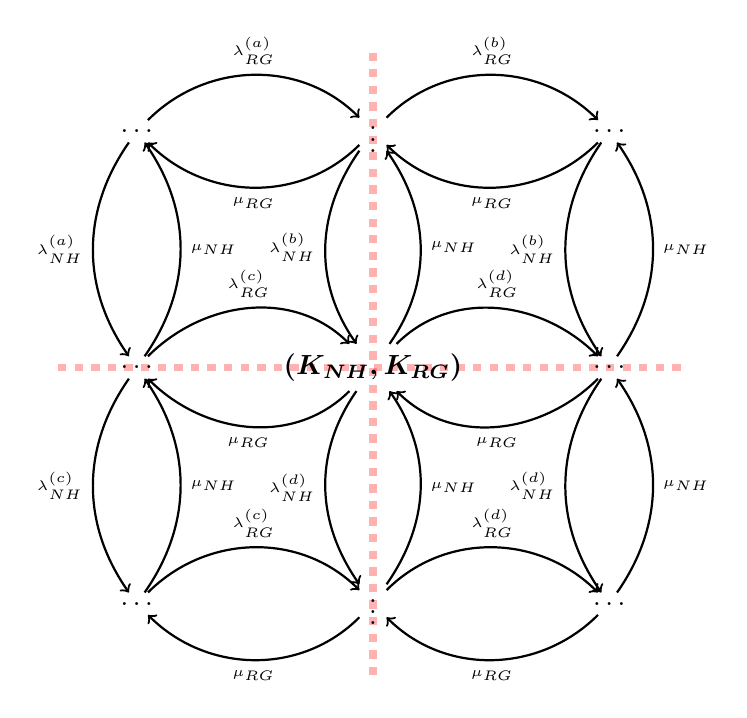
\begin{tikzpicture}[scale=1, every node/.style={scale=1}]
    % -----------------------------------------------
    % Boundaries ------------------------------------
    % -----------------------------------------------
    \draw [dashed, line width=1mm, red, opacity=.3] (2,-3) -- (10,-3);
    \draw [dashed, line width=1mm, red, opacity=.3] (6,1) -- (6,-7);
    %\tikzstyle{state}=[ellipse, draw, fill=blue!10, minimum width=2cm];
    %\tikzstyle{state}=[rectangle, draw, fill=blue!10, minimum width=2cm];
    \tikzstyle{state}=[minimum width=2cm, font=\boldmath];

    % -----------------------------------------------
    % Fourth row--------------------------------------
    % -----------------------------------------------
    \node (ellipsisd1) at ($(0,0) + (3,0)$) {$\dots$};
    \node(dk) at ($(ellipsisd1) + (3,0)$) {$\vdots$};
    \node (ellipsisd2) at ($(dk) + (3,0)$) {$\dots$};
    % Transitions -----------------------------------
    % On Row:
    \draw (ellipsisd1) edge[out=45,in=135,->,thick] node [above] {\tiny$\lambda_{\RG}^{(a)}$} (dk);
    \draw (ellipsisd1) edge[out=-45,in=-135,<-,thick] node [below] {\tiny$\mu_{\RG}$} (dk);

    \draw (dk) edge[out=45,in=135,->,thick] node [above] {\tiny$\lambda_{\RG}^{(b)}$} (ellipsisd2);
    \draw (dk) edge[out=-45,in=-135,<-,thick] node [below] {\tiny$\mu_{\RG}$} (ellipsisd2);

    % -----------------------------------------------
    % Fifth row--------------------------------------
    % -----------------------------------------------
    \node (ellipsise1) at ($(0,-3) + (3,0)$) {$\dots$};
    \node(ek) [state] at ($(ellipsise1) + (3,0)$) {$(K_{\NH},K_{\RG})$};
    \node (ellipsise2) at ($(ek) + (3,0)$) {$\dots$};
    % Transitions -----------------------------------
    % On Row:
    \draw (ellipsise1) edge[out=45,in=135,->,thick] node [above] {\tiny$\lambda_{\RG}^{(c)}$} (ek);
    \draw (ellipsise1) edge[out=-45,in=-135,<-,thick] node [below] {\tiny$\mu_{\RG}$} (ek);

    \draw (ek) edge[out=45,in=135,->,thick] node [above] {\tiny$\lambda_{\RG}^{(d)}$} (ellipsise2);
    \draw (ek) edge[out=-45,in=-135,<-,thick] node [below] {\tiny$\mu_{\RG}$} (ellipsise2);

    % With previous row:

    \draw (ellipsisd1) edge[out=-125,in=125,->,thick] node [left] {\tiny$\lambda_{\NH}^{(a)}$} (ellipsise1);
    \draw (ellipsisd1) edge[out=-55,in=55,<-,thick] node [right] {\tiny$\mu_{\NH}$} (ellipsise1);

    \draw (dk) edge[out=-125,in=125,->,thick] node [left] {\tiny$\lambda_{\NH}^{(b)}$} (ek);
    \draw (dk) edge[out=-55,in=55,<-,thick] node [right] {\tiny$\mu_{\NH}$} (ek);

    \draw (ellipsisd2) edge[out=-125,in=125,->,thick] node [left] {\tiny$\lambda_{\NH}^{(b)}$} (ellipsise2);
    \draw (ellipsisd2) edge[out=-55,in=55,<-,thick] node [right] {\tiny$\mu_{\NH}$} (ellipsise2);
    % Sixth row--------------------------------------
    \node (ellipsisf1) at ($(3,-3) + (0,-3)$) {$\dots$};
    \node(fk) at ($(ellipsisf1) + (3,0)$) {$\vdots$};
    \node (ellipsisf2) at ($(fk) + (3,0)$) {$\dots$};
    % Transitions -----------------------------------
    % On Row:

    \draw (ellipsisf1) edge[out=45,in=135,->,thick] node [above] {\tiny$\lambda_{\RG}^{(c)}$} (fk);
    \draw (ellipsisf1) edge[out=-45,in=-135,<-,thick] node [below] {\tiny$\mu_{\RG}$} (fk);

    \draw (fk) edge[out=45,in=135,->,thick] node [above] {\tiny$\lambda_{\RG}^{(d)}$} (ellipsisf2);
    \draw (fk) edge[out=-45,in=-135,<-,thick] node [below] {\tiny$\mu_{\RG}$} (ellipsisf2);

    % With previous row:

    \draw (ellipsise1) edge[out=-125,in=125,->,thick] node [left] {\tiny$\lambda_{\NH}^{(c)}$} (ellipsisf1);
    \draw (ellipsise1) edge[out=-55,in=55,<-,thick] node [right] {\tiny$\mu_{\NH}$} (ellipsisf1);

    \draw (ek) edge[out=-125,in=125,->,thick] node [left] {\tiny$\lambda_{\NH}^{(d)}$} (fk);
    \draw (ek) edge[out=-55,in=55,<-,thick] node [right] {\tiny$\mu_{\NH}$} (fk);

    \draw (ellipsise2) edge[out=-125,in=125,->,thick] node [left] {\tiny$\lambda_{\NH}^{(d)}$} (ellipsisf2);
    \draw (ellipsise2) edge[out=-55,in=55,<-,thick] node [right] {\tiny$\mu_{\NH}$} (ellipsisf2);

    \end{tikzpicture}
    }
\end{center}
}

\frame{
$$
A =
\begin{pmatrix}
(U_{\NH}(1,1)-t)^2&\dots&(U_{\NH}(1,c_{\RG})-t)^2\\
(U_{\NH}(2,1)-t)^2&\dots&(U_{\NH}(2,c_{\RG})-t)^2\\
\vdots&\ddots&\vdots\\
(U_{\NH}(c_{\NH},1)-t)^2&\dots&(U_{\NH}(c_{\NH},c_{\RG})-t)^2\\
\end{pmatrix}
$$
\vspace{1cm}
$$
B =
\begin{pmatrix}
(U_{\RG}(1,1)-t)^2&\dots&(U_{\RG}(1,c_{\RG})-t)^2\\
(U_{\RG}(2,1)-t)^2&\dots&(U_{\RG}(2,c_{\RG})-t)^2\\
\vdots&\ddots&\vdots\\
(U_{\RG}(c_{\RG},1)-t)^2&\dots&(U_{\RG}(c_{\RG},c_{\RG})-t)^2\\
\end{pmatrix}
$$
}

\frame{

\textbf{Theorem.}\\
Let $f_{h}(k):[1,c_{\bar h}]\to[1,c_h]$ be the best response of player $h\in\{\NH, \RG\}$ to the diversion threshold of $\bar h\ne h$ ($\bar h\in\{\NH, \RG\}$).

If $f_{h}(k)$ is a non-decreasing function in $k$ then the game has at least one Nash Equilibrium in Pure Strategies.\\
}

\frame{
\begin{center}
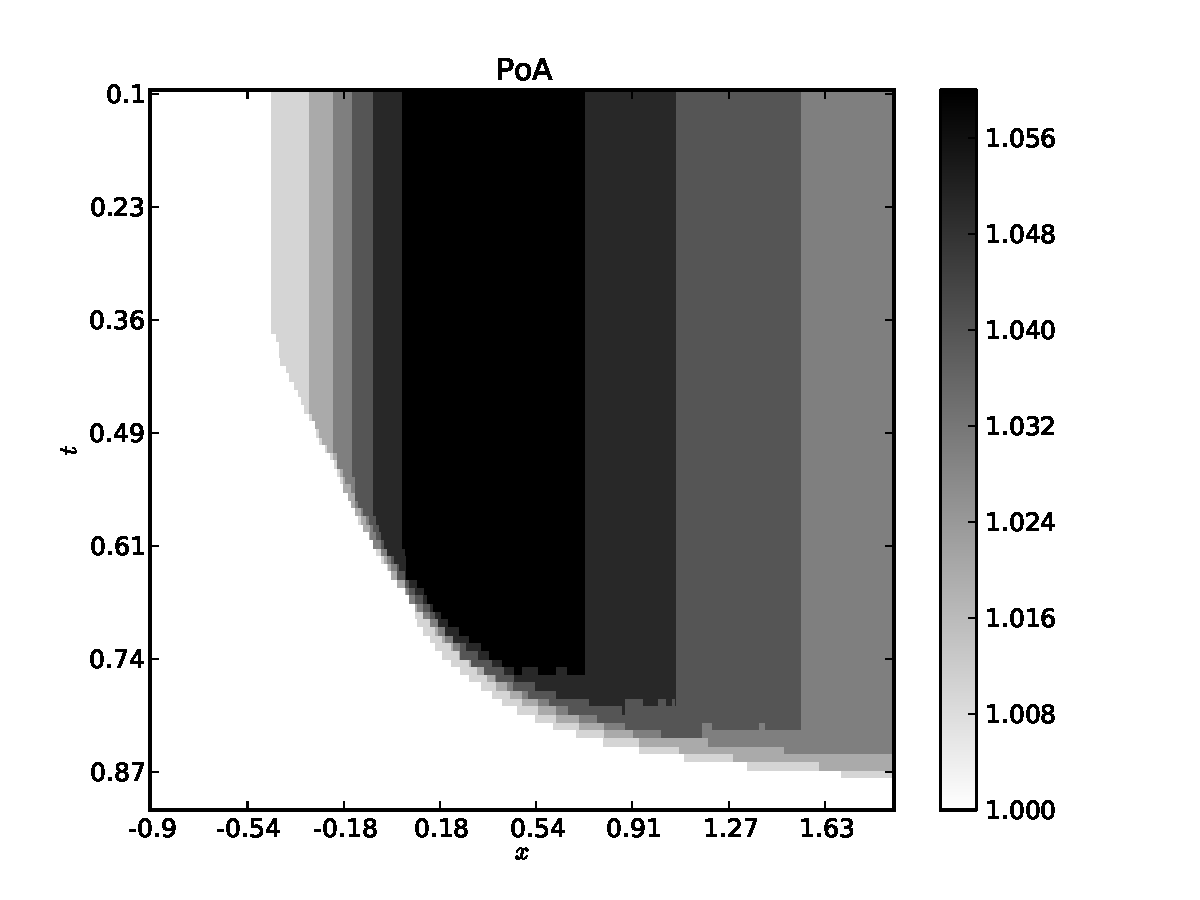
\includegraphics[width=.8\textwidth]{./Images/model2targetvdemand.pdf}
\end{center}
}

\frame{
\begin{center}
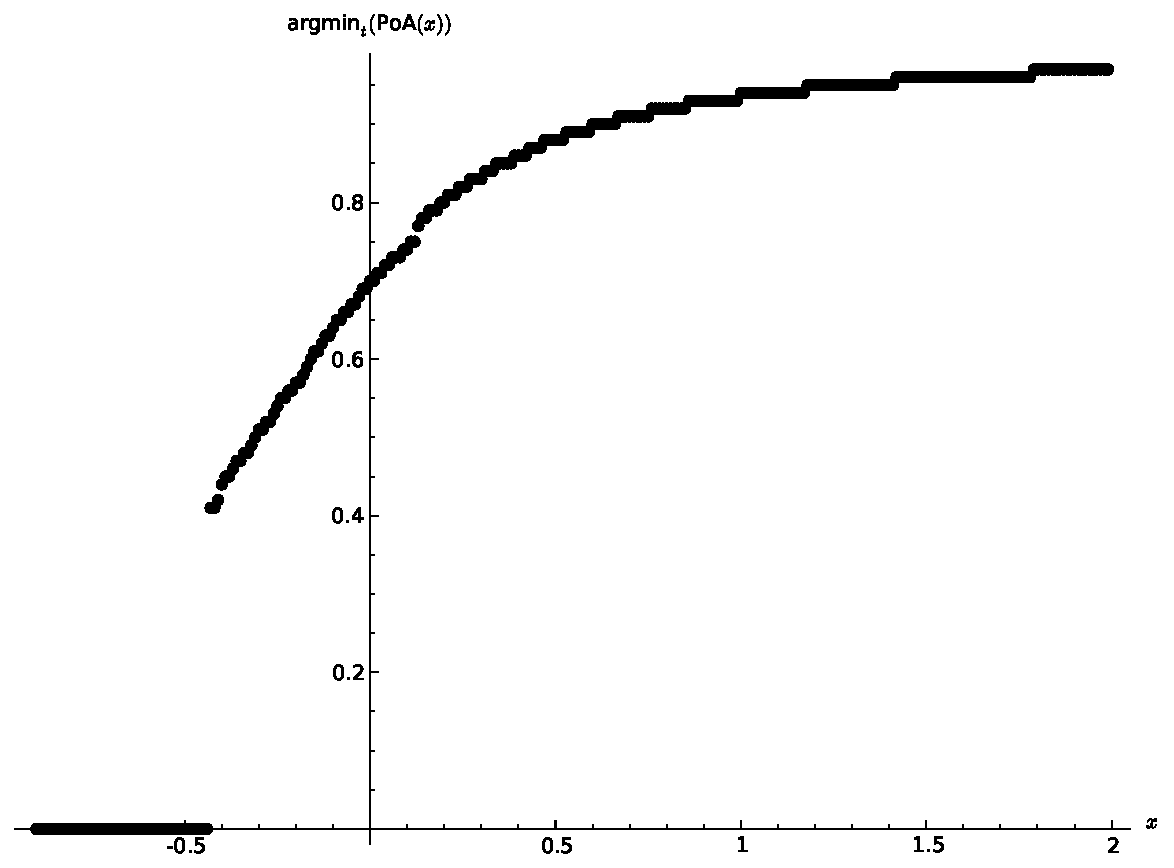
\includegraphics[width=.8\textwidth]{./Images/argminPoAmodel2.pdf}
\end{center}
}

\frame{
    \textbf{Measuring the Price of Anarchy in Critical Care Unit Interactions}, \textit{Submitted to OMEGA}

}

\frame{
    \begin{center}
        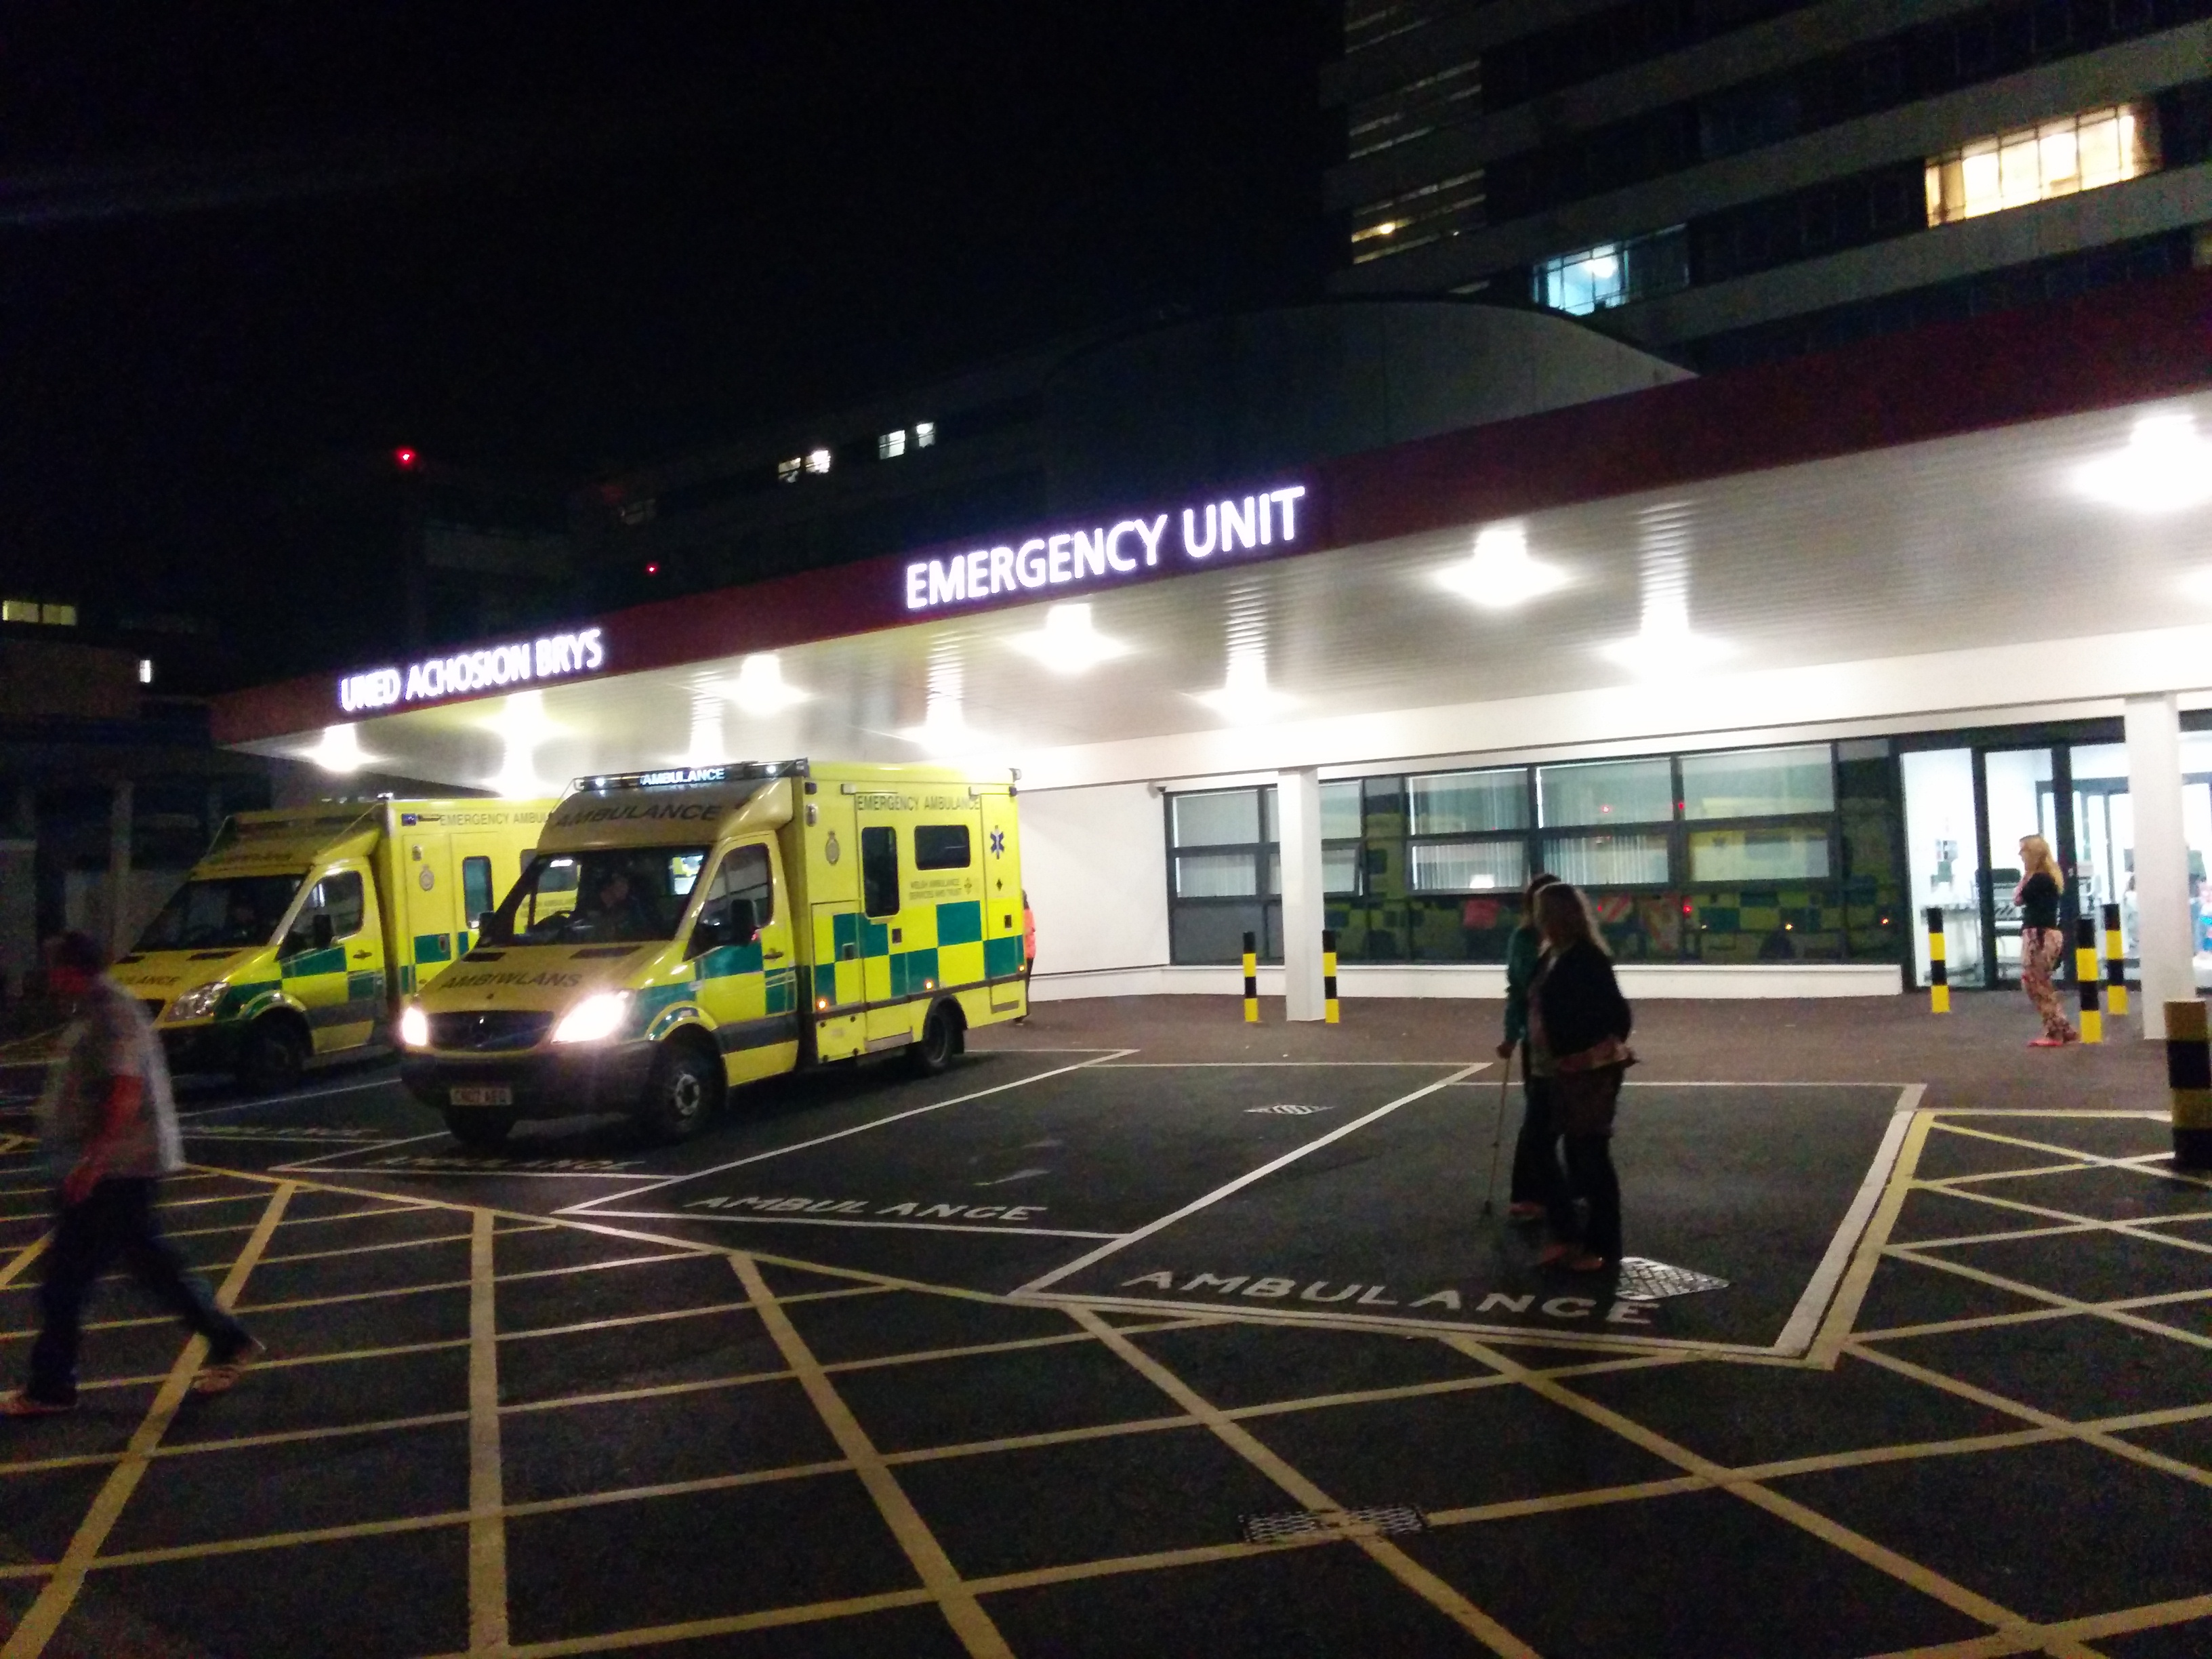
\includegraphics[width=.9\textwidth]{./Images/photo.jpg}
    \end{center}
}

\frame{
    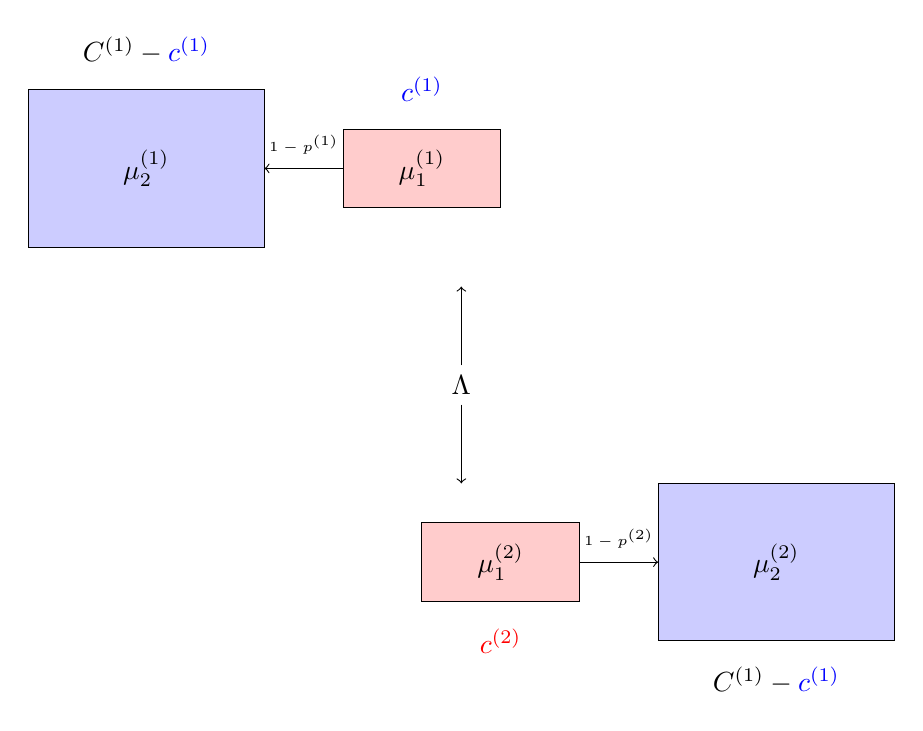
\begin{tikzpicture}
        % First hospital
        \draw [fill=blue!20] (0,0) rectangle (3,2);
        \draw [fill=red!20] (4,.5) rectangle (6,1.5);
        \draw [<-] (3,1) -- (4,1);
        \node at (3.5, 1.3) {\tiny{$1-p^{(1)}$}};
        \node at (1.5,2.5) {$C^{(1)} - \color{blue}{c^{(1)}}$};
        \node at (5,2) {\color{blue}{$c^{(1)}$}};
        \node at (1.5,1) {$\mu_2^{(1)}$};
        \node at (5,1) {$\mu_1^{(1)}$};

        % Second hospital
        \draw [fill=red!20] (5,-3.5) rectangle (7,-4.5);
        \draw [fill=blue!20] (8,-3) rectangle (11,-5);
        \draw [<-] (8,-4) -- (7,-4);
        \node at (7.5, -3.7) {\tiny{$1-p^{(2)}$}};
        \node at (6,-5) {$\color{red}{c^{(2)}}$};
        \node at (9.5,-5.5) {$C^{(1)} - \color{blue}{c^{(1)}}$};
        \node at (6,-4) {$\mu_1^{(2)}$};
        \node at (9.5,-4) {$\mu_2^{(2)}$};

        % Ambulance
        \node at (5.5,-1.75) {$\Lambda$};
        \draw [->] (5.5,-1.5) -- (5.5,-.5);
        \draw [->] (5.5,-2) -- (5.5,-3);
    \end{tikzpicture}
}

\frame{
\begin{center}
\tikzstyle{level 1}=[level distance=4cm, sibling distance=3.5cm]
\tikzstyle{level 2}=[level distance=4cm, sibling distance=2cm]
\tikzstyle{level 3}=[level distance=4cm, sibling distance=1cm]
\tikzstyle{Hosp} = [text width=4em, text centered]
\tikzstyle{end} = [circle, minimum width=3pt,fill, inner sep=0pt]
\begin{tikzpicture}[grow=right, sloped, scale=.8]
\node[Hosp] {$H_1$}
    child {node[Hosp] (a1) {$H_2$}
        child {node[Hosp] (c1) {Am}
            child {node[end, label=right:{$H_2$}] {}}
            child {node[end, label=right:{$H_1$}] {}}
            edge from parent
            node[above] {$C^{(2)} - 1$}
            edge from parent coordinate[pos=1] (b31)
        }
        child {node[Hosp] (c1) {Am}
            child {node[end, label=right:{$H_2$}] {}}
            child {node[end, label=right:{$H_1$}] {}}
            edge from parent
            node[above] {$1$}
            edge from parent coordinate[pos=1] (b41)
        }
        edge from parent
        node[above] {$C^{(1)} - 1$}
        edge from parent coordinate[pos=0.8] (a11)
    }
    child {node[Hosp] (a2) {$H_2$}
        child {node[Hosp] (c1) {Am}
            child {node[end, label=right:{$H_2$}] {}}
            child {node[end, label=right:{$H_1$}] {}}
            edge from parent
            node[above] {$C^{(2)} - 1$}
            edge from parent coordinate[pos=1] (b11)
            }
        child {node[Hosp] (c1) {Am}
            child {node[end, label=right:{$H_2$}] {}}
            child {node[end, label=right:{$H_1$}] {}}
            edge from parent
            node[above] {$1$}
            edge from parent coordinate[pos=1] (b21)
            }
        edge from parent
            node[above] {$1$}
        edge from parent coordinate[pos=0.8] (a21)
    };
\draw[bend right] (a11) to (a21);
\draw[bend right] (b11) to (b21);
\draw[bend right] (b31) to (b41);
\draw[dashed] (a1) to(a2);
\end{tikzpicture}
\end{center}
}

\frame{
    \begin{center}
        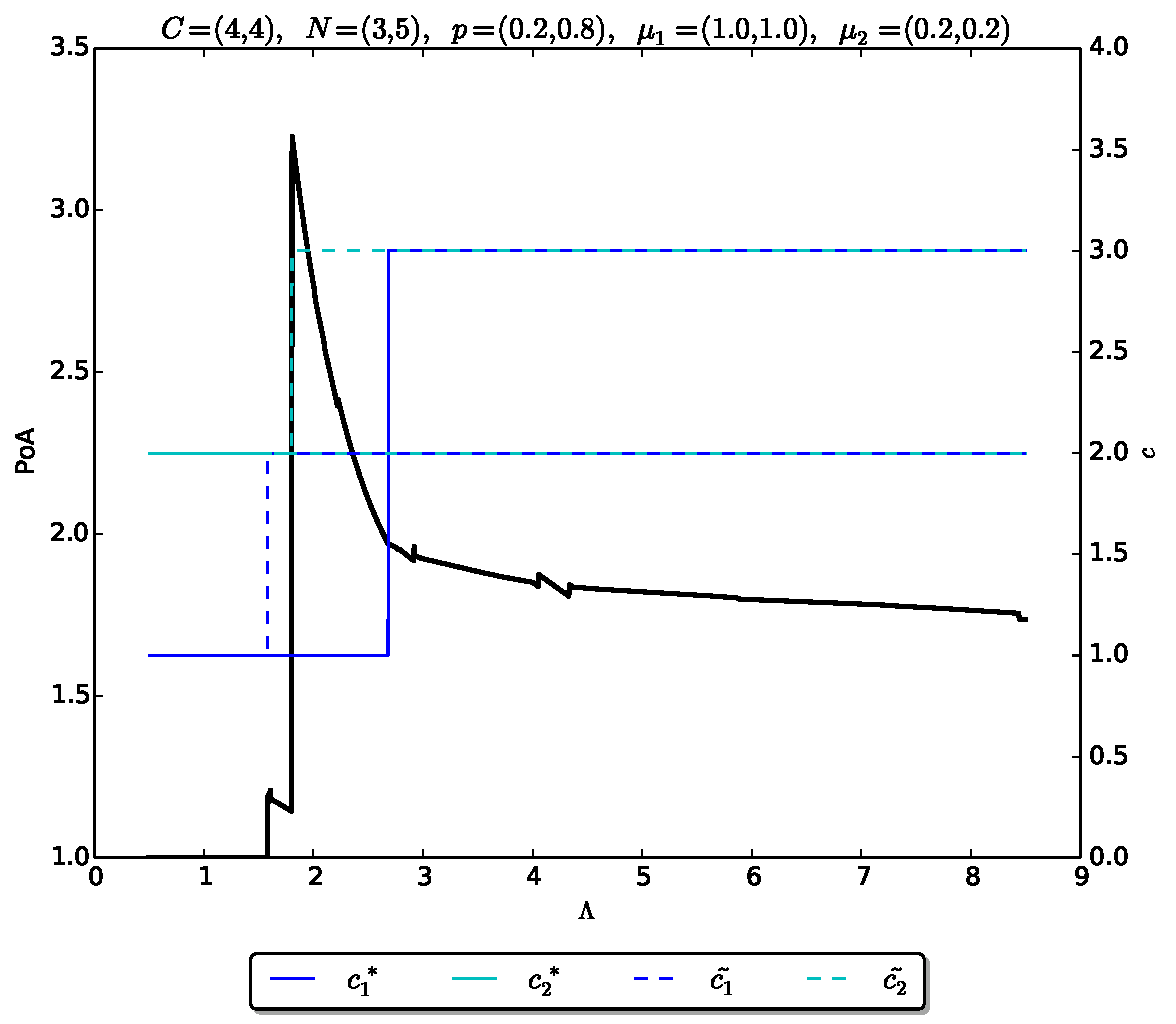
\includegraphics[width=.9\textwidth]{./Images/CCCC-76W.pdf}
    \end{center}
}

\frame{
\begin{center}
\href{https://plus.google.com/+VincentKnight/posts}{+Vincent.Knight}\\
\href{https://twitter.com/drvinceknight}{@drvinceknight}\\
\framebox{\href{http://drvinceknight.github.io/Talks/}{vincent-knight.com/Talks}}
\end{center}
}

\end{document}
